\documentclass[9pt]{beamer}
\usefonttheme{professionalfonts}

\usetheme{Boadilla}
\usecolortheme{whale}
\setbeamertemplate{navigation symbols}{}%remove navigation symbols
\usenavigationsymbolstemplate{}
\setbeamerfont{section number projected}{family=\rmfamily,series=\bfseries,size=\normalsize}
\setbeamercolor{section number projected}{bg=black,fg=yellow}
\setbeamerfont{subsection number projected}{family=\rmfamily,series=\bfseries,size=\normalsize}
\setbeamercolor{subsection number projected}{bg=black,fg=yellow}
\setbeamertemplate{sections/subsections in toc}[square]
\usepackage{amsmath,amsthm,amssymb,mathdots}
\usepackage{mathtools} %% pmatrix*
%% \usepackage{fourier}
\usepackage{multicol}
\usepackage{multirow}
% \usepackage[table]{xcolor}    
%\usepackage{fontspec}
\usepackage{bbding}
\usepackage{subfigure}
%\usepackage[most]{tcolorbox}
\newcounter{testexample}
\usepackage{xparse}
\usepackage{lipsum}
\usepackage[UTF8,noindent]{ctex}
\usepackage{extarrows}
\usepackage{array}
%% \usepackage{courier}
\usepackage{animate}
\usepackage{dcolumn}
\usepackage[ruled,vlined,linesnumbered]{algorithm2e}
\usepackage[]{hyperref}
\usepackage{pgf}
%% \usepackage{pgfplots}
\usepackage[framemethod=TikZ]{mdframed}
\usepackage{tikz}
\usetikzlibrary{calc,shapes.multipart,chains}
\usetikzlibrary{arrows,snakes,backgrounds,shapes,patterns,shadows}
\usetikzlibrary{matrix,fit,positioning,decorations.pathmorphing}
%% \usepackage{calligraphy}
%% \usepackage{matrixcells}
%% \usepackage{tikzamsmatrix}
\usepackage{color, colortbl}
\usepackage{cases}
\usepackage{enumerate}

\usepackage{listings}
\lstset{
        language=python,
        keywordstyle=\color{red},
        % frame=single,
        basicstyle=\ttfamily,
        commentstyle=\color{blue},
        breakindent=0pt,
        rulesepcolor=\color{red!20!green!20!blue!20},
        rulecolor=\color{black},
        tabsize=4,
        numbersep=5pt,
        breaklines=true,
        %backgroundcolor=\color{red!15},
        showstringspaces=false,
        showspaces=false,
        showtabs=false,
        extendedchars=false,
        escapeinside=``,
}
\tikzset{mystyle/.style n args={5}{
    rectangle,
    draw,
    fill=#1!50,
    % rounded corners,
    minimum height=#2cm,
    minimum width=#3cm,
    text width=#4cm,
    align=#5
  }}

\tikzset{mystyle1/.style n args={5}{
    rectangle,
    fill=#1!50,
    minimum height=#2cm,
    minimum width=#3cm,
    text width=#4cm,
    align=#5
  }}

\tikzset{mystyle2/.style n args={5}{
    rectangle,
    % draw,
    fill=#1!30,
    % rounded corners,
    minimum height=#2,
    minimum width=#3\textwidth,
    text width=#4\textwidth,
    align=#5
  }}


\tikzset{myarrow/.style n args={2}{
    ->,
    #1,
    line width=#2
  }}

\tikzset{list/.style={
rectangle split,
rectangle split parts=2,
rectangle split horizontal,
rectangle split part fill={red!30,blue!20},
rounded corners,
node distance=.5cm,
draw=black, thick,
minimum height=0.35cm,
text width=.5cm,
text centered,
}}

\tikzset{dlist/.style args={#1}{
rectangle split,
rectangle split parts=3,
rectangle split horizontal,
rectangle split part fill={blue!20,red!30,blue!20},
rounded corners,
node distance=#1mm,
draw=black, thick,
minimum height=0.35cm,
text centered,
}}

\tikzset{sentinel/.style args={#1}{
rectangle split,
rectangle split parts=3,
rectangle split horizontal,
rectangle split part fill={white,white,white},
rounded corners,
node distance=#1mm,
draw=black, thick,
minimum height=0.35cm,
text centered,
}}

\tikzset{square/.style args={#1}{
rectangle,draw,
fill=#1!30,
minimum height=.35cm,
minimum width=.35cm
}}

\usepackage{refcount}
\usepackage{multicol}
\newcounter{countitems}
\newcounter{nextitemizecount}
\newcommand{\setupcountitems}{%
        \stepcounter{nextitemizecount}%
        \setcounter{countitems}{0}%
        \preto\item{\stepcounter{countitems}}%
}
\makeatletter
\newcommand{\computecountitems}{%
        \edef\@currentlabel{\number\c@countitems}%
        \label{countitems@\number\numexpr\value{nextitemizecount}-1\relax}%
}
\newcommand{\nextitemizecount}{%
        \getrefnumber{countitems@\number\c@nextitemizecount}%
}
\newcommand{\previtemizecount}{%
        \getrefnumber{countitems@\number\numexpr\value{nextitemizecount}-1\relax}%
}
\makeatother    
\newenvironment{AutoMultiColItemize}{%
        \ifnumcomp{\nextitemizecount}{>}{3}{\begin{multicols}{2}}{}%
                \setupcountitems\begin{itemize}}%
                {\end{itemize}%
                \unskip\computecountitems\ifnumcomp{\previtemizecount}{>}{3}{\end{multicols}}{}}


%% If you build your own environment using array, you're on the safe side. I would extend an int%% ernal macro of amsmath using an optional argument.
%%
%% Advantages:
%%
%% It extends several matrix environments at the same time (matrix, pmatrix, bmatrix, Bmatrix, vmatrix, Vmatrix).
%%
%% The names and meanings of those environments remain (not apmatrix etc.)
%%
%% Spacing etc. is the same like in amsmath.
%%
%% You could do more than just insert a vertical line (use color and alignment, for instance right aligned columns because of minus signs).
%%
%% If you omit the optional argument, it acts exactly like the amsmath environment.
%%
%% Caution:
%%
%% Since you redefine an internal macro, it might not work if the original package changes its code. But amsmath.sty has not been changed for more than 10 years. If there's a change in the matrices later, you could adjust your own macro.
%% Code:
%% Here's the redefinition, just put it in your preamble after loading amsmath:
\makeatletter
\renewcommand*\env@matrix[1][*\c@MaxMatrixCols c]{%
  \hskip -\arraycolsep
  \let\@ifnextchar\new@ifnextchar
  \array{#1}}
\makeatother

%% Examples:

%% Simple augmented matrix:

%% \begin{pmatrix}[cc|c]
%%   1 & 2 & 3\\
%%   4 & 5 & 9
%% \end{pmatrix}
%% More complex use, with different alignment, spacing and color:

%% \begin{bmatrix}[*2cr@{\quad}|@{\quad}>{\color{red}}r]
%%   a & b & 1  &  4 \\
%%   c & d & -2 & -3
%% \end{bmatrix}

% ######### DEFINE COLOR ###############
\definecolor{blue}{rgb}{0.0,0.0,1.0}
\definecolor{red}{rgb}{1.0,0.0,0.0}
\definecolor{purple}{rgb}{0.75, 0.0, 1.0}
\definecolor{LightCyan}{rgb}{0.88,1,1}

\def\blue{\textcolor{blue}}
\def\red{\textcolor{red}}
\def\purple{\textcolor{purple}}

\newcommand\aug{\fboxsep=-\fboxrule\!\!\!\fbox{\strut}\!\!\!}

\def\argmax{\mathop{\arg\max}}
\def\lst{\lstinline}
\def\ds{\displaystyle}
\def\cd{\cdots}
\def\dd{\ddots}
\def\vd{\vdots}
\def\id{\iddots}
\def\ft{\frametitle}
\def\diag{\mathrm{diag}}
\def\Im{\mathrm{Im~}}
\def\Ker{\mathrm{Ker~}}
\def\r{\mathrm{R}}
\def\rank{\mathrm{rank}}
\newcommand{\ttt}[1]{\texttt{#1}}

\def\cA{{\mathcal{A}}}
\def\cB{{\mathcal{B}}}
\def\cC{{\mathcal{C}}}
\def\cD{{\mathcal{D}}}
\def\cE{{\mathcal{E}}}
\def\cF{{\mathcal{F}}}
\def\cG{{\mathcal{G}}}
\def\cH{{\mathcal{H}}}
\def\cI{{\mathcal{I}}}
\def\cJ{{\mathcal{J}}}
\def\cK{{\mathcal{K}}}
\def\cL{{\mathcal{L}}}
\def\cM{{\mathcal{M}}}
\def\cN{{\mathcal{N}}}
\def\cO{{\mathcal{O}}}
\def\cP{{\mathcal{P}}}
\def\cQ{{\mathcal{Q}}}
\def\cR{{\mathcal{R}}}
\def\cS{{\mathcal{S}}}
\def\cT{{\mathcal{T}}}
\def\cU{{\mathcal{U}}}
\def\cV{{\mathcal{V}}}
\def\cW{{\mathcal{W}}}
\def\cX{{\mathcal{X}}}
\def\cY{{\mathcal{Y}}}
\def\cZ{{\mathcal{Z}}}

\def\vA{{\boldsymbol{A}}}
\def\vB{{\boldsymbol{B}}}
\def\vC{{\boldsymbol{C}}}
\def\vD{{\boldsymbol{D}}}
\def\vE{{\boldsymbol{E}}}
\def\vF{{\boldsymbol{F}}}
\def\vG{{\boldsymbol{G}}}
\def\vH{{\boldsymbol{H}}}
\def\vI{{\boldsymbol{I}}}
\def\vJ{{\boldsymbol{J}}}
\def\vK{{\boldsymbol{K}}}
\def\vL{{\boldsymbol{L}}}
\def\vM{{\boldsymbol{M}}}
\def\vN{{\boldsymbol{N}}}
\def\vO{{\boldsymbol{O}}}
\def\vP{{\boldsymbol{P}}}
\def\vQ{{\boldsymbol{Q}}}
\def\vR{{\boldsymbol{R}}}
\def\vS{{\boldsymbol{S}}}
\def\vT{{\boldsymbol{T}}}
\def\vU{{\boldsymbol{U}}}
\def\vV{{\boldsymbol{V}}}
\def\vW{{\boldsymbol{W}}}
\def\vX{{\boldsymbol{X}}}
\def\vY{{\boldsymbol{Y}}}
\def\vZ{{\boldsymbol{Z}}}
\def\v0{{\boldsymbol{0}}}
\def\vLambda{{\boldsymbol{\Lambda}}}

\def\va{{\boldsymbol{a}}}
\def\vb{{\boldsymbol{b}}}
\def\vc{{\boldsymbol{c}}}
%% \def\vd{{\boldsymbol{d}}}
\def\ve{{\boldsymbol{e}}}
\def\vf{{\boldsymbol{f}}}
\def\vg{{\boldsymbol{g}}}
\def\vh{{\boldsymbol{h}}}
\def\vi{{\boldsymbol{i}}}
\def\vj{{\boldsymbol{j}}}
\def\vk{{\boldsymbol{k}}}
\def\vl{{\boldsymbol{l}}}
\def\vm{{\boldsymbol{m}}}
\def\vn{{\boldsymbol{n}}}
\def\vo{{\boldsymbol{o}}}
\def\vp{{\boldsymbol{p}}}
\def\vq{{\boldsymbol{q}}}
\def\vr{{\boldsymbol{r}}}
\def\vs{{\boldsymbol{s}}}
\def\vt{{\boldsymbol{t}}}
\def\vu{{\boldsymbol{u}}}
\def\vv{{\boldsymbol{v}}}
\def\vw{{\boldsymbol{w}}}
\def\vx{{\boldsymbol{x}}}
\def\vy{{\boldsymbol{y}}}
\def\vz{{\boldsymbol{z}}}


\def\bx{{\mathbf{x}}}


\def\R{\mathbb R}
\def\C{\mathbb C}
\def\F{\mathbb F}
\def\dim{\mathrm{dim~}}
\def\tr{\mathrm{tr}}
\def\det{\mathrm{det}}
\def\coef{\mathrm{coef}~}


\def\tf{\ttfamily}
\def\vLambda{\boldsymbol{\Lambda}}
\def\vPhi{\boldsymbol{\Phi}}
\def\vPsi{\boldsymbol{\Psi}}
\def\valpha{\boldsymbol{\alpha}}
\def\vbeta{\boldsymbol{\beta}}
\def\vgamma{\boldsymbol{\gamma}}
\def\vxi{\boldsymbol{\xi}}
\def\vzeta{\boldsymbol{\zeta}}
\def\veta{\boldsymbol{\eta}}
\def\vepsilon{\boldsymbol{\epsilon}}
\def\vphi{\boldsymbol{\phi}}
\def\vvarphi{\boldsymbol{\varphi}}
\def\vsigma{\boldsymbol{\sigma}}
\def\vomega{\boldsymbol{\omega}}
\def\vtau{\boldsymbol{\tau}}
%\def\rank{\boldsymbol{rank}}

\include{asset/global_theorem_fancybox}
\def\exampletext{例} % If English
\NewDocumentEnvironment{testexample}{ O{} }
{
\colorlet{colexam}{red!55!black} % Global example color
\newtcolorbox[use counter=testexample]{testexamplebox}{%
    % Example Frame Start
    empty,% Empty previously set parameters
    title={\exampletext: #1},% use \thetcbcounter to access the testexample counter text
    % Attaching a box requires an overlay
    attach boxed title to top left,
       % Ensures proper line breaking in longer titles
       minipage boxed title,
    % (boxed title style requires an overlay)
    boxed title style={empty,size=minimal,toprule=0pt,top=4pt,left=3mm,overlay={}},
    coltitle=colexam,fonttitle=\bfseries,
    before=\par\medskip\noindent,parbox=false,boxsep=0pt,left=3mm,right=0mm,top=2pt,breakable,pad at break=0mm,
       before upper=\csname @totalleftmargin\endcsname0pt, % Use instead of parbox=true. This ensures parskip is inherited by box.
    % Handles box when it exists on one page only
    overlay unbroken={\draw[colexam,line width=.5pt] ([xshift=-0pt]title.north west) -- ([xshift=-0pt]frame.south west); },
    % Handles multipage box: first page
    overlay first={\draw[colexam,line width=.5pt] ([xshift=-0pt]title.north west) -- ([xshift=-0pt]frame.south west); },
    % Handles multipage box: middle page
    overlay middle={\draw[colexam,line width=.5pt] ([xshift=-0pt]frame.north west) -- ([xshift=-0pt]frame.south west); },
    % Handles multipage box: last page
    overlay last={\draw[colexam,line width=.5pt] ([xshift=-0pt]frame.north west) -- ([xshift=-0pt]frame.south west); },%
    }
\begin{testexamplebox}}
{\end{testexamplebox}\endlist}
\usepackage{tikz-qtree}
\usepackage{tikz}
\usepackage{mathpazo}
\usepackage{pgfplots}
\newcommand{\num}{pi}
\pgfplotsset{compat=1.8}
 % define the plot style and the axis style
\tikzset{elegant/.style={smooth,thick,samples=50,magenta}}

\begin{document}
\title[管理运筹学]{管理运筹学}
\author[DYH]
{董银红}
\institute[]
{
  % \inst{1}
中南民族大学管理学院
}
\date[]
{\today}
\subject{Computational Mathematics}

\frame{
  \titlepage
  % \begin{tikzpicture}[remember picture,overlay]
  %   \node [opacity=.9] at (current page.south west) [above right=1.3cm]{\includegraphics[width=0.15\textwidth]{whu_log.jpeg} };
  %   \node [opacity=.35] at (current page.south) [above] {\includegraphics[width=\textwidth]{ML_log.png} };
  % \end{tikzpicture}
}

\begin{frame}
  \frametitle{目录}
  \tableofcontents[hideallsubsections]
\end{frame}

\AtBeginSection[]
{
  \begin{frame}[shrink]
    \frametitle{目录}
    \tableofcontents[currentsection,hideallsubsections]
  \end{frame}
}

\AtBeginSubsection[]
{
  \begin{frame}
    \frametitle{目录}
    \tableofcontents[currentsection,currentsubsection]
  \end{frame}
} 

%%%%%
\section{引言}

\begin{frame}{\secname}
\begin{itemize}
    \item “运筹于帷幄之中,决胜于千里之外”。运筹学将科学的方法、技术和工具应用到经济管理、工程设计等领域,以便为人们提供最佳的解决方案。
    \item 在这一章里,首先介绍运筹学的基本概况,包括运筹学的历史和发展,运筹学的性质和特点,运筹学研究的主要内容和以后的发展趋势。然后从运筹学问题解决过程的角度,依次介绍建模、求解和实际应用时应该注意的一些问题,使初学者对运筹学概念和方法有初步的认识。
\end{itemize}
\end{frame}

\subsection{运筹学概况}
\subsubsection{运筹学历史}
\begin{frame}[allowframebreaks]{\subsecname}
\begin{itemize}
    \item 运筹学的产生很难有一个明确的时间界定,目前国际上比较公认的观点是运筹学产生于第二次世界大战前后。
    \item 1937年英国部分科学家被邀请去帮助皇家空军研究雷达的部署和运作问题,目的在于最大限度地发挥有限雷达的效用,以应对德军的空袭。
    \item 1938年波德塞(Bawdsey)雷达站的负责人罗伊(Rowe)提出了优化防空作战系统运行的问题,并用“Operational Research”一词作为对这一方面研究的描述,这就是今天仍然将运筹学称为O.R.的历史由来。
    \item 1939年从事此方面问题研究的科学家被召集到英国皇家空军指挥总部,成立了一个由布莱开特(Blacket)领导的军事科技攻关小组;由于其成员学科性质的多样性,这一最早成立的军事科技攻关小组被戏称为“布莱开特马戏团”。由于“布莱开特马戏团”的活动是第一次有组织的系统的运筹学活动,所以后人将该小组的成立作为运筹学产生的标志。
    \item 此后,O.R.小组的活动范围不断扩大,从最初的仅限于空军,逐步扩展到了海军和陆军;研究内容也从对军事战术性问题的研究,逐步扩展到对军事战略性问题的研究。
    \item 由于科学家的天赋、战争的需要以及不同学科的交互作用,这一军事科技攻关小组在提高军事运筹水平方面取得了惊人的成功,这使得运筹学在整个军事领域迅速传播,到1941年英国皇家陆、海、空三军都成立了这样的科学小组。比较典型的论题包括雷达布置策略、反空袭系统控制、海军舰队的编制和对敌潜艇的探测等。
    \item 第二次大战结束以后,美国等国家的军方仍然保留了一些运筹小组,其他的多数人转向把运筹学研究应用于和平时期的工商业。因此美国,德国等国家的运筹学得以蓬勃发展,出现了应用研究和理论研究相互促进的局面。
    \item 从应用方面来讲,在工商业管理中的应用是主要的,特别是在美国,管理科学方面的主要内容便是运筹学。
    \item 从学校教育方面来说,许多大学理学院的数学系及工学院、管理学院、经济学院的许多系中都开设运筹学课程。
    \item 从科学发展来说,在运筹研究或运筹学这一名称下发展起来的分支学科就很多,如规划论(包含线性规划、非线性规划、整数规划、 动态规划、多目标规划等)、网络分析、排队论、对策论、决策论、存储论、可靠性理论、模型论、投入产出分析等等。
从学会方面来说,最早的是美国的运筹学会,成立于1952年。
\end{itemize}
\end{frame}

\subsubsection{运筹学的性质与特点}
\begin{frame}{\subsubsecname}
    运筹学是一门综合性应用型学科,也是上个世纪形成的一门科学。当人们把战时的运筹研究取得成功的经验在和平时期加以推广应用时,面临着一个广阔的研究领域。
\begin{itemize}
    \item 科学性:运筹学原理中引进了大量的数学研究方法。
\item 系统性:运筹学研究问题是从系统的观点出发,研究全局性的问题,研究综合优化的规律,它是系统工程的主要理论基础。
\item 应用性:在运筹学术界,有许多人强调运筹学的实用性和对研究结果的执行效果,并把执行效果看作运筹工作中的一个很重要的组成部分。
\item 跨学科性:
早期运筹学小组都是由不同领域的专家组成。
\item 理论和应用相互促进,相得益彰。
运筹学的各个分支学科,都是由于实际问题的需要或以一定的实际问题为背景逐渐发展起来的。
\end{itemize}
\end{frame}

\subsubsection{运筹学的主要内容}
\begin{frame}{\subsubsecname}
\begin{itemize}
    \item 运筹学的发展历史不算太长,但是其内容丰富,涉及面广,应用范围大,已经形成了一个相当庞大的学科。它的主要内容一般应该包含线性规划、非线性规划、整数规划、动态规划、多目标规划、随机规划、网络分析、排队论、对策论、 决策论、存储论、可靠性理论、模型论、投入产出分析等。它们中的每一部分都可以独立成册,都有丰富的内容。
    \item 上述的前六个部分统称为规划论,它们主要是解决两个方面的问题。一个方面的问题是对于给定的人力、物力和财力,怎样才能发挥他们的最大效益; 另一个方面的问题就是对于给定的任务,怎样才能用最少的人力、物力和财力去完成它。
\end{itemize}
\end{frame}

\subsection{运筹学问题的求解过程}
\begin{frame}{\subsecname}
    既然运筹学的使命是要解决问题,那么怎么样去解决呢?解决问题可以定义为:识别问题,确定备选方案,实施方案和评价方案这四个最基本的流程。那么运筹学问题的解决对应着从现实系统到模型,模型的求解,模型结论所提供的方案,现实结论以及实现效果。作为研究对象的系统来说,总是要求我们求解一定的未知量并给出相应的结论,求解过程如图\ref{fig:ch1-1}所示。图中虚线表示了人们最直接的目标,右侧的实线表示了这一目标的具体实现路径。
\begin{figure}[htbp]\label{fig:ch1-1}
  \centering
  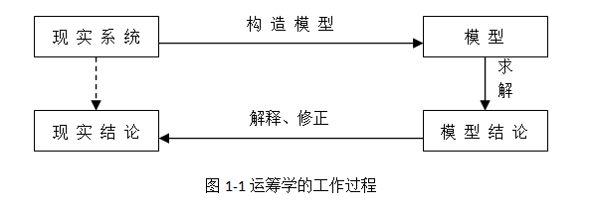
\includegraphics[width=5 in,height=2 in]{pic/1_1.png}
  \caption{运筹学的工作过程}
\end{figure}
\end{frame}

\subsubsection{从现实系统到理论模型:模型建立}
\begin{frame}[allowframebreaks]{\subsubsecname}
\begin{enumerate}
    \item 模型是现实世界的抽象化反映。运筹学的实质在于建立和使用模型来解决实际问题。尽管模型的具体结构和形式总是与要解决的问题相联系,但在这里将抛弃模型在外表上的差别,从最广泛的角度抽象出它们的共性。模型在某种意义上说是客观事物的简化与抽象,是研究者经过思维抽象后用文字、图表、符号、关系式以及实体模样对客观事物的描述。
    \item 模型有三种基本类型,即形象模型、模拟模型和数学模型。
\begin{itemize}
    \item 物理复制被称为形象模型,比如孩子的卡车,飞机模型等等。
\item 模拟模型也是物理模型,但是在外形上与被建模的对象并不一样,比如汽车上的速度表就是一种模拟模型。
\item 模型的第三种类型是数学模型,它是以一些系统化的符号和数学表达式或关系式来反映实际问题。
\end{itemize}
\item 运筹学模型主要是指数学模型。\\
数学模型可以简单的描述为:用字母、数字和运算符来精确地反映变量之间相互关系的式子或式子组。
数学模型由决策变量、约束条件和目标函数三个要素构成。决策变量即问题中所求的未知的量,约束条件是决策所面临的限制条件,目标函数则是衡量决策效益的数量指标。
一旦所有可控和非可控输入都已经确定,目标函数和约束条件就可在模型中被考虑,模型的输出便也确定下来。这样的话,模型的输出就是在那些实际环境因素和决策下会产生的结果了。图1-2表示的是数学模型如何将可控和非可控输入转化为结果输出以及这个生产模型的具体细节。

\begin{figure}\label{fig:ch1-2}
  \centering
  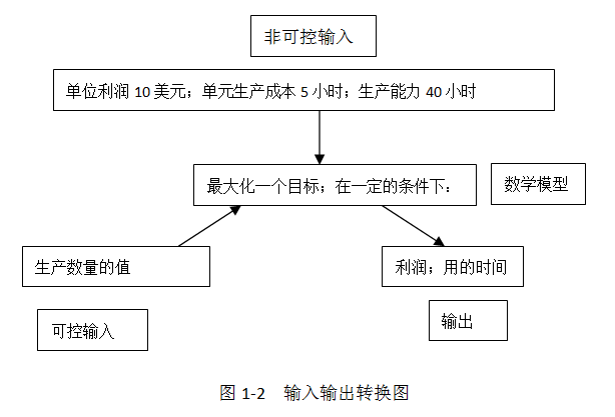
\includegraphics[width=4 in,height=3 in]{pic/1_2.png}
  \caption{}
\end{figure}
\begin{itemize}
    \item 非可控输入既可以是非常明确的,也可以是不确定的、变化的。
\item 如果一个模型的非可控输入都是已知的、不可变的,这样的模型称为确定模型。
\item 如果一个模型的非可控输入是不确定的、变化的,这样的模型就称为随机模型或概率模型。
\item 本书主要研究确定型数学模型。
\end{itemize}
\end{enumerate}
\end{frame}

\begin{frame}{\subsubsecname}
  了解模型的相关概念之后,下一个问题就是如何将一个现实问题转化为数学模型,也就是建模过程。既然运筹学模型的几个要素是:目标函数,约束条件(包括自然约束和强加约束),决策变量。那么根据我们要解决的问题,只要我们经常问自己下面这些问题,一个模型的框架是不难建立的。

\begin{itemize}
    \item 我们需要什么目标?
    \item 通过调节哪些因素可以使得我们达到这一目标?
    \item 调节的因素是变动的吗? 
    \item 要与实际情况相符合有什么限制条件吗?
     \item 在实现目标的过程中,有哪些约束条件?
      \item 这样建立的模型是相对完备的吗?
\end{itemize}

\end{frame}

\begin{frame}{\subsubsecname}
对以上问题的回答只是提供了一种建立模型的基本框架结果,对于数学规划类的建模,这种思路也是很有效的。一个问题解决的好坏,与建立的模型和所使用的工具关系是相当密切的。数学模型不可能完全刻画现实世界,正如经济学诺贝尔奖获得者和计算机图灵奖获得者,著名的决策理论专家所言,数学模型并不要求准确无误,它只需要尽可能接近地给出比靠常识得到更好的解就可以了。
\end{frame}

\subsubsection{模型到方案:模型的求解}
\begin{frame}{\subsubsecname}
    \begin{itemize}
        \item 一旦建模和数据准备工作已经完成,我们就可以进入模型求解阶段。在此阶段分析人员将确定决策变量的具体值,以获得模型的最优输出结果。这些具体的决策变量的值,或者说能够得到最优输出结果的值,通常称为模型的最优解。对于前面的生产问题来说,模型的求解阶段包括,找到能实现最大化利润,同时又不违反生产能力约束条件的决策变量(生产数量)的值。
\item 模型求解的过程中可能会用到一种反复实验的方法。通过对提供的一些备选方案进行测试评估,可以得到满足条件的较好方案。如果某个方案不能满足其中的一个或多个约束条件,那么无论目标函数的值是多少,这个方案都是不可行的,从而不能被采纳。如果所有的约束条件都满足了,那么它就是可行解,或者说是备选项。
\item 整个运筹学的学习,就是要有效率地解决问题,模型和算法的好坏直接影响了这一目标的实现。对于算法的设计,方法有很多,在我们运筹学的学习中,主要是强调迭代法。尽管问题千差万别,但是具体的步骤却是差不多的。为了更形象的说明这一步骤,我们不妨举个例子。你现在要到一个地方。这个时候你可能会考虑以下几个问题:
\begin{itemize}
    \item (1)我现在在哪里?
\item (2)我将要去哪里?
\item (3)朝哪个方向走?
\item (4)选择每步走多大的一步?
\end{itemize}
    \end{itemize}
\end{frame}

\begin{frame}{\subsubsecname}
一个迭代算法的思想和我们要去一个地方这一目标的思想是一致的。在设计一个迭代算法的时候,我们依然是考虑这四个问题。迭代算法主要就是通过当前点到下一个点的变化来实现。先找到当前点,这是我们的新的起点,然后通过一定的规则到达下一个点,以下一个点为当前点,继续后面的过程直至终止。对应上面四个问题,我们考虑的是:
\begin{itemize}
\item (1)初始点(我现在在哪里);
\item (2)终止准则(我们的目标是什么);
\item (3)迭代方向(朝哪个方向走);
\item (4)迭代步长(选择每步都多远)。
\end{itemize}
\end{frame}

\subsubsection{从结果到结论}
\begin{frame}{\subsubsecname}
   通过计算机或者手工得到的最优解不一定我们需要的结论。通过定量计算求解只是决策的一部分工作,还不是作为管理者和决策者要的结论。决策者需要的是可以具体实施的简单易行的报告。报告除了推荐的方案和一些有助于决策的相关信息,所推荐的方案不仅在理论上能够说服别人,在实践上也是简单可行的。所以在使用软件的同时,更重要的是能够正确的解读软件给我们的结果。在具体的问题中,我们将继续探讨这一问题。
\end{frame}



\begin{frame}{矩阵表示}
$$
\begin{gathered}
    \begin{matrix}
    0&1 \\ 1&0
    \end{matrix}
    \quad
    \begin{pmatrix}
    0 &-i \\ i &0
    \end{pmatrix}
    \quad
    \begin{bmatrix}
    0 & -1\\1&0
    \end{bmatrix}
\end{gathered}
$$
\end{frame}
\section{线性规划简介}
\begin{frame}{\secname}
\begin{itemize}
    \item 线性规划是运筹学中研究最早,理论和算法比较成熟的一个重要分支,其应用十分广泛。
    \item 早在1939年,前苏联的数学家康托洛维奇(1975年诺贝尔经济学获得者)就提出了生产组织和管理中的线性规划模型。
    \item 20世纪40年代末,美国的Dantzig提出了求解一般线性规划的单纯形方法。Charnes对于线性规划的理论和应用也作出了突出的贡献。
    \item 目前可供计算大规模线性规划问题的计算机软件也较为成熟。因此,线性规划在工农业生产、商业活动、军事行动和科学研究的各个方面都得到了重要的应用。
\end{itemize}
 \end{frame}
 
 \subsection{线性规划模型}
\begin{frame}{\subsecname}
    %在了解线性规划的理论和应用前,必须先对线性规划模型有一个形象的映像。这一节将继续绪论中的讨论,首先介绍如何将真实问题转化为数学模型。下面通过两个示例(最优投资组合问题和投资决策问题)来介绍这一问题。
 \begin{example}[2-1:投资组合问题]
 一个投资者希望用一定数量的资金进行投资。他对10种不同的股票进行投资,并估计在1年内投资的收益。表2-1给出了每种股票的国别、风险类别(R为高风险,N为低风险)和期望投资收益率(ROI)。投资者确定了某些约束条件。为了分摊风险,他希望对每种股票的投资最多占总资金的30%。进一步,他希望资金的一半能够投资在北美的股票和最多 是高风险投资。这些资金应该怎样在各种股票中进行分配才能达到最大化的收益的目的呢?
 
 % Please add the following required packages to your document preamble:
% \usepackage[table,xcdraw]{xcolor}
% If you use beamer only pass "xcolor=table" option, i.e. \documentclass[xcolor=table]{beamer}
\begin{table}[]
\begin{tabular}{|c|c|c|c|c|}
\hline
\textbf{编号} & \textbf{描述} & \textbf{国别} & \textbf{风险类型} & \textbf{期望收益率} \\ \hline
\rowcolor[HTML]{FFFFFF} 
1           & 国库券         & 加拿大         & N             & 5              \\ \hline
\rowcolor[HTML]{FFFFFF} 
2           & 硬件          & 美国          & R             & 17             \\ \hline
\rowcolor[HTML]{FFFFFF} 
3           & 剧院          & 美国          & R             & 26             \\ \hline
\rowcolor[HTML]{FFFFFF} 
4           & 电信          & 美国          & R             & 12             \\ \hline
\rowcolor[HTML]{FFFFFF} 
5           & 酿酒          & 英国          & N             & 8              \\ \hline
\rowcolor[HTML]{FFFFFF} 
6           & 高速公路        & 法国          & N             & 9              \\ \hline
\rowcolor[HTML]{FFFFFF} 
7           & 汽车          & 德国          & N             & 7              \\ \hline
\rowcolor[HTML]{FFFFFF} 
8           & 银行          & 卢森堡         & N             & 6              \\ \hline
\rowcolor[HTML]{FFFFFF} 
9           & 软件          & 印度          & R             & 31             \\ \hline
\rowcolor[HTML]{FFFFFF} 
10          & 电子          & 日本          & R             & 21             \\ \hline
\end{tabular}
\end{table}
 \end{example}   
\end{frame}

\begin{frame}{\secname}
    解:为了构建数学模型,首先要确定问题的解中包含的决策变量:在当前的案例中,希望知道整个投资中每种股票的投资数量。因此,定义决策变量 表示股票 在投资资金中所占的比例。这也就意味着所有变量都必须是一个在0和1之间的分数(其中1代表整个资金的100\%)。事实上,每个变量都有一个最大值约束,即投资者期望的投资每种股票最多占整个资金的30\%。以下约束条件建立了所有变量的边界:
$$
0 \le x_i \le \frac{1}{3}, \quad i=1,2,\dots, 10.
$$
将$w_i$ 作为股票$i$的期望ROI,在这里表示:
$$
w=(5,17,26,12,8,9,7,6,31,21)
$$
投资者希望将所有的资金都进行投资,也就是说不同股票的分数之和必须为100%。这可以表达为以下等式约束:
$$
\sum_{i=1}^{10} x_i =1
$$
\end{frame}

\begin{frame}{\subsecname}
现在仍然需要两个约束条件来表达投资者的特殊要求。至多1/3的资金是高风险股票,即投资到这个类型股票的资金之和不能超过整个资金的1/3:
$$
x_2+x_3+x_4+x_9+x_{10} \le \frac{1}{3}
$$
投资者同样坚持对北美的股票的投资最少50%:
$$
x_1+x_2+x_3+x_4 \ge \frac{1}{2}
$$
这两个约束条件为不等式约束。
    投资者的目标是最大化所有股票投资的收益,也就是说最大化下面的表达式:
$$
\sum_{i=1}^{10} w_ix_i
$$
这就是数学模型的目标函数。
\end{frame}

\begin{frame}{\subsecname}
\begin{block}{线性规划模型}
可以得到以下整个数学模型的表达式:
\begin{alignat}{2}
&&\min\quad   \sum_{i=1}^{10} w_i x_i \\
\mbox{s.t.}\quad
\left\{
\begin{array}{cc}
     & \sum_{i=1}^{10} x_i =1 \\
     & x_2+x_3+x_4+x_9+x_{10} \le \frac{1}{3}\\
     & x_1+x_2+x_3+x_4 \ge \frac{1}{2} \\
     & x_i \ge 0, \quad i=1,2,\cd, 10.
\end{array}
\right.
\end{alignat}
\end{block}
\end{frame}

\begin{frame}{\subsecname}
通过对这个问题的解读,已经将以上的模型建立起来了。其中,“maximize”表示最大化。S.t.是英文“subject to”的缩写,“使得”的意思。下面来回忆一下整个建模过程和线性规划的一些特点:
\begin{itemize}
    \item 全面了解问题。
     \item 描述目标。
\item 描述约束条件。
\item 定义决策变量。
\item 用决策变量写出目标和约束条件。
\end{itemize}
以上问题就是线性规划模型或者线性规划。正如前面所述,该问题有目标和约束条件,这是所有线性规划所共有的特点。并且它的目标函数和约束条件都是关于决策变量的线性函数。线性函数是指函数中的每个变量都是分离的并且幂次为1。在刚才的模型中,目标函数是线性函数,因为所有的决策变量都是分离的,并且都是一次幂。约束条件的左边都是线性函数,因此称此问题为线性规划。

线性规划有3个基本的假设:比例性、可加性和可分性。比例性是指目标函数值和约束条件所对应的资源值与决策变量值成比例。可加性是指目标函数的值和使用资源总量分别可以通过汇总所有的决策变量对目标函数的贡献和各个决策变量使用资源数量而得到。可分性是指决策变量是连续的。非负条件和可分性假设意味着决策变量可以是大于或者等于零的一切数值。

\end{frame}

\begin{frame}{\subsecname}

      \begin{example}
      某公司有100万的资金可供投资。该公司有六个可选的投资项目,其各自的数据如表2-2所示:
% Please add the following required packages to your document preamble:
% \usepackage[table,xcdraw]{xcolor}
% If you use beamer only pass "xcolor=table" option, i.e. \documentclass[xcolor=table]{beamer}
\begin{table}[]
\begin{tabular}{|c|c|c|c|c|}
\hline
\textbf{投资项目} & \textbf{风险(\%)} & \textbf{红利(\%)} & \textbf{增长率(\%)} & \textbf{信用度} \\ \hline
\rowcolor[HTML]{FFFFFF} 
1             & 18             & 4              & 22              & 4            \\ \hline
\rowcolor[HTML]{FFFFFF} 
2             & 6              & 5              & 7               & 10           \\ \hline
\rowcolor[HTML]{FFFFFF} 
3             & 10             & 9              & 12              & 2            \\ \hline
\rowcolor[HTML]{FFFFFF} 
4             & 4              & 7              & 8               & 10           \\ \hline
\rowcolor[HTML]{FFFFFF} 
5             & 12             & 6              & 15              & 4            \\ \hline
\rowcolor[HTML]{FFFFFF} 
6             & 8              & 8              & 8               & 6            \\ \hline
\end{tabular}
\end{table}
      该公司想达到的目标为:投资风险最小,每年的红利至少为6.5万元,最低平均增长率为12\%,最低平均信用度为7。
      \end{example}

\end{frame}

\begin{frame}{\subsecname}
    解:首先面对这一问题,要抓住决策变量、目标以及约束条件。
    \begin{itemize}
        \item \red{决策变量}:本问题的决策变量是在每种投资项目上的投资额。设$X_i$为项目i的投资额。
        \item \red{目标函数}:本问题要求总投资最小,即:
        $$
        \min \quad z=0.18x_1+0.06x_2+0.1x_3+0.04x_4+0.12x_5+0.08x_6
        $$
        \item \red{约束条件}:本问题共有5个约束条件。这些约束可以表示为:
        \begin{itemize}
            \item 各项目投资总额为100万: \\ $x_1+x_2+x_3+x_4+x_5+x_6=100$.
            \item 每年的红利至少为6.5万:\\
            $0.04x_1+0.05x_2+0.09x_3+0.07x_4+0.06x_5+0.08x_6 \ge 6.5$.
            \item 最低平均增长率为12\%:\\
        $0.22x_1+0.07x_2+0.12x_3+0.08x_4=0.15x_5+0.08x_6 \ge 100\times 12\%$
           \item 最低平均信用度为7: \\
           $4x_1+10x_2+2x_3+10x_4+4x_5+6x_6 \ge 7 \times 100$
           \item 非负约束:\\
           $x_1, x_2,x_3,x_4,x_5,x_6 \ge 0$
        \end{itemize}
    \end{itemize}
\end{frame}

\begin{frame}{\subsecname}
  
    \begin{block}{数学模型}  
    于是得到以下的线性规划模型:
\begin{alignat}{2}
\min\quad  z=0.18x_1+0.06x_2+0.1x_3+0.04x_4+0.12x_5+0.08x_6 \nonumber\\
\mbox{s.t.}\quad
\left\{
\begin{array}{cc}\nonumber
     & x_1+x_2+x_3+x_4+x_5+x_6=100 \\
     & 0.04x_1+0.05x_2+0.09x_3+0.07x_4+0.06x_5+0.08x_6 \ge 6.5\\
     & 0.22x_1+0.07x_2+0.12x_3+0.08x_4=0.15x_5+0.08x_6 \ge 100\times 12\% \\
     & 4x_1+10x_2+2x_3+10x_4+4x_5+6x_6 \ge 7 \times 100 \\
     & x_i \ge 0, \quad i=1,2,\cd, 6.
\end{array}
\right.
\end{alignat}
\end{block}

\begin{alertblock}{注:}
  这是一个典型的成本(或者风险)最小化问题。模型的意义是在给定的限制条件下,求使得目标函数达到最小时的每个项目投资额。可以看到,以上问题是线性规划模型。该问题有目标和约束条件,其目标函数和约束条件都是决策变量的线性函数,也满足线性规划的3个基本假设。
\end{alertblock}

\end{frame}

\subsection{图解法}
\begin{frame}{\subsecname}
    对模型中只含有2个变量的线性规划问题,可以通过在平面上作图的方法求解。通过图解法,可以对线性规划问题及其求解过程有一个直观的认识,便于建立N维空间中线性规划问题的概念,同时帮助读者更好地理解求解一般线性规划问题的单纯形法的思路。
\end{frame}

\subsubsection{线性规划问题图解法的步骤}
\begin{frame}{\subsubsecname}
    为了便于理解,下面将通过抽象出来的数学规划模型来具体说明线性规划问题图解法的步骤,以便理解。
    \begin{example}[例2-3] 
    考虑只有两个变量的线性规划问题,用图解法解答:
    \begin{alignat}{2}
\min\quad  z=x_1+3x_2 \nonumber\\
\mbox{s.t.}\quad
\left\{
\begin{array}{cc}\nonumber
     & x_1+x_2 \le 6 \\
     & 2x_1-x_2 \ge 0\\
     & x_2 \le 3\\
     & x_i \ge 0, \quad i=1,2.
\end{array}
\right.
\end{alignat}
    \end{example}
\end{frame}

\begin{frame}{\subsubsecname}
\begin{itemize}
    \item 在平面上建立直角坐标系
    \item 根据图示约束条件,找出可行域
     \item 图示目标函数
     \item 寻找最优解
\end{itemize}
    最优解的目标函数值为:
    $$
    z=x_1+3x_2=3+3\times 3 = 12
    $$
\end{frame}

\begin{frame}{\subsubsecname}
\centering
       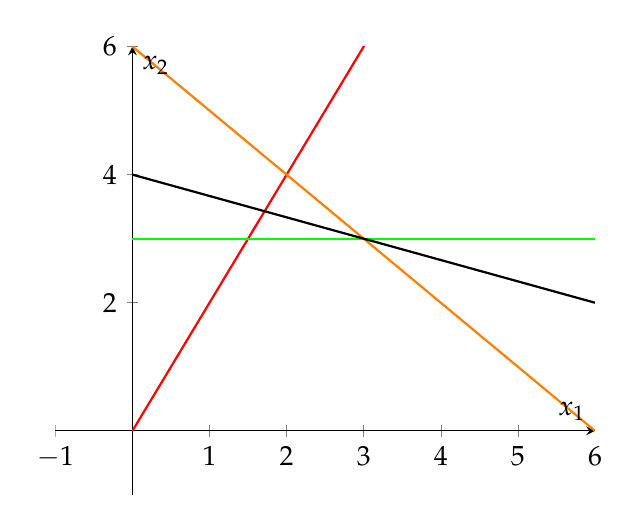
\begin{tikzpicture}
    % the axis environment 
    \begin{axis}[axis x line=middle,
                 axis y line=middle,
                 xmin=-1,xmax=6,
                 ymin=-1,ymax=6,
                 ylabel=$x_2$,
                 xlabel=$x_1$]
        \addplot[elegant,red,domain=0:12]{2*x};
        \addplot[elegant,green,domain=0:10]{3};
        \addplot[elegant,orange,domain=0:6]{6-x};
       \addplot[elegant,black,domain=0:6]{-1/3*x+4};
    \end{axis}
\end{tikzpicture}

\end{frame}

\subsubsection{线性规划解的情况}
\begin{frame}{\subsubsecname}
  \begin{itemize}
    \item 有唯一的最优解
    \item  有无穷多最优解
    \item 无界解
    \item  无解,或无可行解
\end{itemize}  
\begin{figure}\label{fig:ch2-2}
  \centering
  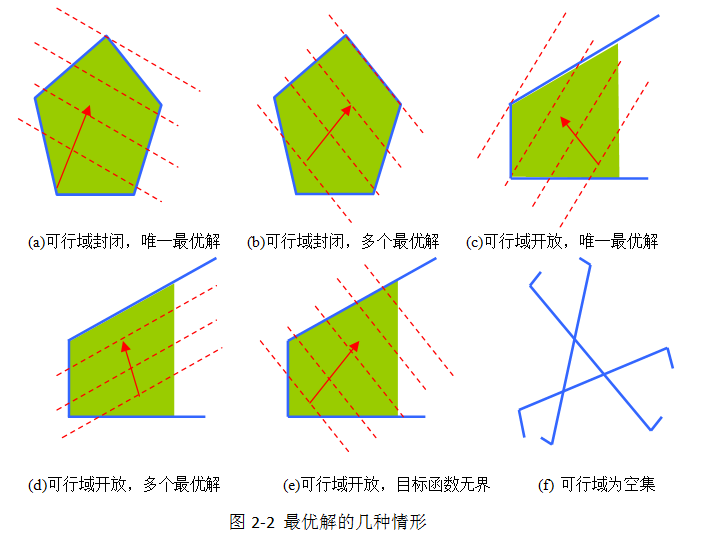
\includegraphics[width=4 in,height=2.5 in]{pic/2_2.png}
  \caption{最优解的几种情形}
\end{figure}
\end{frame}

\subsubsection{线性规划问题的标准形式}
\begin{frame}{\subsubsecname}
 由于目标函数和约束条件在内容与形式上的差别,导致线性规划问题表达多种多样,为了便于讨论线性规划问题的求解方法和解的性质,需要规定线性规划问题的标准形式。如果一个线性规划问题满足以下条件,就称为标准形式的线性规划问题:
 \begin{enumerate}
        \item 求目标函数的最大值;
        \item 所有变量均要求取非负值;
        \item 所有的约束条件(变量非负约束除外)必须为等式;
        \item 约束条件右端常数项$b_i$全为非负值。
\end{enumerate}
\end{frame}

\begin{frame}{\subsubsecname}
    \begin{alignat}{2}
\max \quad  z=\sum_{j=1}^n c_jx_j \nonumber\\
\mbox{s.t.}\quad
\left\{
\begin{array}{cc}\nonumber
     & \sum_{j=1}^n a_{i,j}x_j=b_i \quad i=1,2,\cd, m\\
     & x_j \ge 0, \quad j=1,2, \cd, m.
\end{array}
\right.
\end{alignat}
标准形式的矩阵表达式如下:
 \begin{alignat}{2}
\max \quad  z=c^Tx \nonumber\\
\mbox{s.t.}\quad
\left\{
\begin{array}{cc}\nonumber
     & \vA X = b\\
     & x_j \ge 0, \quad j=1,2, \cd, m.
\end{array}
\right.
\end{alignat}
其中,
$$
\begin{gathered}
   c=
    \begin{bmatrix}
    c_1 \\c_2 \\ \vdots \\c_n
    \end{bmatrix}
    \quad
  X= \begin{bmatrix}
    x_1 \\x_2 \\ \vdots \\x_n
    \end{bmatrix}
    \quad
  b= \begin{bmatrix}
    b_1 \\b_2 \\ \vdots \\x_m
    \end{bmatrix}
    \vA=
    \begin{bmatrix}
    a_{11}&a_{12}&\cd &a_{1n}\\
    a_{21}&a_{22}&\cd &a_{2n}\\
    \cd &\cd& \cd &\cd\\
    a_{m1}&a_{m2}&\cd &a_{mn}
    \end{bmatrix}
\end{gathered}
$$
\end{frame}

\subsection{线性规划的基本概念}
\begin{frame}{\subsecname}
    对于各种非标准形式的线性规划问题,总可以通过以下的变换,将其转化为标准形式。
\begin{itemize}
    \item[(1)] 极小化目标函数的问题:
\item[(2)] 约束条件不为等式的问题:
\item[(3)] 变量无符号限制的问题:
\item[(4)] 变量小于等于零的问题:
\end{itemize}
\end{frame}

\subsubsection{线性规划问题的解}
\begin{frame}{\subsubsecname}
    在图解法中,已经比较直观地讨论了线性规划问题的可行解和最优解等概念,但图解法无法解决三个及其三个变量以上的线性规划问题,为了用代数方法求得可行域的极点,还需要引入以下一些有关线性规划可行域和解的概念。
\begin{definition}[超平面]
在n维空间中,满足条件:
$
a_{i1}x_1+a_{i2}x_2+ \cd +a_{in}x_n=b_i
$
的点集$X=(x_1,x_2,\cd,x_n)^T$ 称为一个\red{超平面}。
\end{definition}
\begin{definition}[半空间]
在n维空间中,满足条件:
$
a_{i1}x_1+a_{i2}x_2+ \cd +a_{in}x_n \le (或者 \ge ) b_i
$
的点集$X=(x_1,x_2,\cd,x_n)^T$ 称为一个\red{半空间}。
\end{definition}
\begin{definition}[多面体]
有限个半空间的交集,即同时满足以下条件的非空点集:
$$
a_{i1}x_1+a_{i2}x_2+ \cd +a_{in}x_n\le (或 \ge ) b_i
,\quad i=1,2,\cd, m 
$$
的点集$X=(x_1,x_2,\cd,x_n)^T$ 称为一个\red{多面体}。
\end{definition}
\end{frame}

\begin{frame}{\subsubsecname}

\begin{definition}[线性规划的基]
对于线性规划的约束条件
$$
\vA X=b
$$
$$
X \ge 0
$$
其中$\vA$为$m\times n$的矩阵,$n>m$,秩$\vA=m$,$b$为$ m \times 1$向量。设$\vB$是$\vA$矩阵中的一个非奇异的$m\times m$子矩阵,则称$\vB$为线性规划的一个\red{基}。
\end{definition}

\begin{definition}[基解、基可行解和可行基]
线性规划的解:
$$
X=\begin{bmatrix}
X_B \\ X_N
\end{bmatrix}
=\begin{bmatrix}
B^{-1}b \\ 0
\end{bmatrix}
$$
称为线性规划与基$\vB$对应的基解。
\end{definition}
\end{frame}

\section{线性规划的计算机求解}
\subsection{用Excel“规划求解”功能求解线性规划}
\begin{frame}{\subsecname}
\begin{itemize}
    \item 在Excel电子表格中建立线性规划模型
    \item 利用Excel“规划求解”功能求解线性规划问题
    \begin{itemize}
        \item “Set Target”(设置目标单元格):在这一栏中,输入表示目标函数值的单元格地址“B10”(也可以直接单击B10单元格)。
        \item “Equal to”(等于):选中“min”;
        \item 在“By changing cells:”中输入:B4:G4表示决策变量的位置。
        \item 在“subject to the constraints”一栏中通过“Add”添加约束条件。
        (5)单击“Options”按钮,在弹出的“Solver Options”对话框中,设置求解运算中的有关参数。本问题需要选择“Assume Linear Model”和“Assume Non-Negative”。这是采用线性模型和假定非负的复选框,单击确定;
\item 单击左上角的“Solve”按钮,则开始进行规划求解。
\item 在弹出的“Solver Results”对话框中(注意:当模型没有可行解或者目标值为无穷的时候,规划求解结果的内容将不同),选中“keep Solver Solution”,保存结果,单击“OK”。
    \end{itemize}
\end{itemize}
\end{frame}

\subsubsection{用LINDO/LINGO求解线性规划问题}
\begin{frame}{用LINDO求解线性规划问题}
    安装好LINDO软件包以后,点击执行文件。此时会弹出LINDO软件的空白对话框。在空白对话框中就可以直接书写命令了。\\
下面给出其结果的一般解释:
\begin{itemize}
    \item “LP OPTIMUM FOUND AT STEP 3”表示LINDO 在(用单纯形法)3次迭代或旋转后得到最优解。
    \item “OBJECTIVE FUNCTION VALUE 1) 8.25”表示最优目标值为8.25。
“VALUE”给出最优解中各变量的值。
\end{itemize}
要得到以上结果,必须遵循以下简单的软件规则:
\begin{itemize}
    \item (1) 目标函数及各约束条件之间一定要有“Subject to (ST) ”分开。
\item (2) 变量名不能超过8个字符。
\item (3) 变量与其系数间可以有空格,单不能有任何运算符号(如乘号“*”等)。
\item (4) 要输入<=或>=约束,相应以<或>代替即可。
\item (5) 一般LINDO 中不能接受括号“()“和逗号“,“,例:400(X1+X2) 需写成400X1+400X2;10,000 需写成10000。
\item (6) 表达式应当已经简化过。不能出现 2 X1+3 X2-4 X1,而应写成-2X1+3 X2。
\end{itemize}

\end{frame}

\begin{frame}{LINGO软件求解线性规划}
    LINGO是求解优化问题的一个专业工具软件,它包含了内置的建模语言,容许用户以简单直观的方式描述较大规模的优化模型,对于模型中所需要的数据可以以一定的形式保存在独立的文件中,读取也很方便快捷。
    
    一般来说,在LINGO中建立优化模型都是由四个部分组成,也即是:集合段,数据段,初始段以及目标与约束段。每个模型都是由model语句开始,由end语句结束。
    
\end{frame}

\section{线性规划的单纯型算法}

\begin{frame}{\secname}
\begin{itemize}
    \item  图解法只能求解比较简单的线性规划形式,利用计算机求解虽然能够解决大规模的线性规划问题,但是掩盖了实际的求解方法和过程。为了更深入地学习线性规划和开发新的算法,必须要对线性规划的求解机理有一定的了解。
\item 本章在对线性规划的模型有一定认识后,从代数形式上继续考察线性规划问题。首先,给出线性规划相关的一些概念和最优解的性质;然后,在此基础上提出单纯形原理;在对单纯形法进行完整描述后,本章将对单纯形法提出了进一步的说明。通过本章的学习,读者应该对线性规划的单纯形的思想和步骤有较为清晰的理解。
\end{itemize}
\end{frame}

\subsection{线性规划的基本理论}
\begin{frame}{可行区域的几何结构}
考虑标准的线性规划问题:
$$
\min c^Tx
$$
$$
Ax=b,\quad x\ge 0
$$
用$R^n$ 表示n维的欧式空间,这里$\vx \in R^n$, $c\in R^n$, $b\in R^n$, $\vA \in R^{m\times n}$. 不妨设可行区域$\vD=\{x\in R^n \mid \vA \vx=b, x\ge 0\}\neq \Phi$,因此线性方程组      相容,总可以把多余方程去掉,使剩下的等式约束的系数向量线性无关,故可设$秩(\vA)=m$,$m<n$。

\end{frame}












\begin{frame}{\secname} 
  \begin{definition}[行秩 \& 列秩]
    \begin{itemize}
    \item      
      $\vA$的行向量组的秩,称为矩阵$\vA$的\red{行秩}。
    \item
      $\vA$的列向量组的秩,称为矩阵$\vA$的\red{列秩}。
    \end{itemize}      
  \end{definition}
  \pause 
  \begin{alertblock}{注}
    对于$m\times n$阶矩阵$\vA$,其行秩$\le m$,列秩$\le n$。
  \end{alertblock}
\end{frame}

\begin{frame}{\secname}
  
  \begin{definition}[阶梯型矩阵]
    若矩阵$\vA$满足
    \begin{itemize}
    \item[(1)] 零行在最下方;
    \item[(2)] 非零行首元的列标号随行标号的增加而严格递增,
    \end{itemize}
    则称$\vA$为\red{阶梯型矩阵}。
  \end{definition}
  \begin{example}
    $$
    \left(
    \begin{array}{rrrr}
      2&3&2&1\\
      0&5&2&-2\\
      0&0&3&2\\
      0&0&0&0
    \end{array}
    \right)
    $$
  \end{example}
  
\end{frame}


\begin{frame}{\secname}
  
  \begin{definition}[行简化阶梯型矩阵]
    若矩阵$\vA$满足
    \begin{itemize}
    \item[(1)] 它是阶梯型矩阵;
    \item[(2)] 非零首元为$1$;
    \item[(3)] 非零行首元所在的列除其自身外,其余元素全为零,
    \end{itemize}
    则称$\vA$为\red{行简化阶梯型矩阵}。
  \end{definition}
  \begin{example}
    $$
    \begin{pmatrix*}[r]
      1&2&0& 1&0&3\\
      0&0&1&-2&0&4\\
      0&0&0& 0&1&5\\
      0&0&0& 0&0&0
    \end{pmatrix*}
    $$
  \end{example}
  
\end{frame}



%\section{对偶线性规划与灵敏度分析}

\subsection{变分法,哈密尔顿动力系统}

\begin{frame}{\subsecname}
\begin{definition}[拉格朗日量]
定义光滑函数
\begin{equation}\label{eq:lagrange}
    L: \R^n \times \R^n \to \R, \quad
    L = L(\vx, \vv), 
\end{equation}
称之为\red{拉格朗日量}. 
\end{definition}
\pause 

设$T > 0$,$\vx^0, \vx^1 \in \R^n$已知。
\begin{block}{变分法研究的基本问题(变分问题)}
求曲线$\vx^*: [0, 1] \to \R^n$以极小化泛函
\begin{equation}\label{eq:cvp}
    I[\vx(\cdot)] = \int_0^T L(\vx(t), \dot\vx(t))\,dt, 
\end{equation}
对所有满足条件$\vx(0)=\vx^0, \vx(T)=\vx^1$的函数$\vx(\cdot)$。
\end{block}
\end{frame}

% \subsubsection{欧拉-拉格朗日方程}
\begin{frame}{\subsecname}
    对拉格朗日量$L=L(\vx,\vv)$,将变量$\vx$看做是位置,将$\vv$看做是速度。记
    $$
    \frac{\partial L}{\partial x_i} = L_{x_i}, \quad
    \frac{\partial L}{\partial v_i} = L_{v_i}
    $$
    及
    $$
    \nabla_{\vx} L = 
    \begin{bmatrix}
    L_{x_1} & \cd & L_{x_n}
    \end{bmatrix}^T, \quad 
    \nabla_{\vv} L = 
    \begin{bmatrix}
    L_{v_1} & \cd & L_{v_n}
    \end{bmatrix}^T. 
    $$
    
    \pause 
    \begin{theorem}[欧拉-拉格朗日方程]
    设$\vx^*(\cdot)$为变分问题\eqref{eq:cvp}的解,则$\vx^*(\cdot)$必为\red{欧拉-拉格朗日方程}
    \begin{equation}\label{eq:EL}
        \frac{d}{dt} \left[\nabla_{\vv} L(\vx(t),\vv(t))\right] = \nabla_{\vx} L(\vx(t),\vv(t))
    \end{equation}
    的解。
    \end{theorem}
    \pause 
    \begin{block}{注}
    \begin{itemize}
    \item 若能求解欧拉-拉格朗日方程,则原变分问题的解(若存在)必在这些解中。
   \item 欧拉-拉格朗日方程是一个拟线性系统,它含$n$个二阶常微分方程,其中第$i$个方程可表示为
   \begin{equation}
       \frac{d}{dt} \left[L_{v_i}(\vx(t), \dot\vx(t))\right] = L_{x_i}(\vx(t), \dot\vx(t)).
   \end{equation}
    \end{itemize}

    \end{block} 
\end{frame}

\begin{frame}{\subsecname}
    \begin{block}{证明.}
    \begin{enumerate}
        \item 对任意光滑函数$\vy: [0,T]\to \R^n, \vy(0)=\vy(T)=\v0$,定义
        $$
        i(\tau) := I[\vx^*(\cdot) + \tau\vy(\cdot)], \quad \forall \tau \in \R.
        $$
        由于$\vx^*(\cdot)$为极小值点,故
        $$
        i(\tau) \ge i(0) = I[\vx^*(\cdot)] .
        $$
        即$i(\tau)$在$\tau=0$处取到极小值,从而
        $$
        i^\prime(0) = 0.
        $$
    \end{enumerate}
    \end{block}
\end{frame}

\begin{frame}{\subsecname}
    \begin{block}{证明.【续】}
    \begin{enumerate}[2]
        \item 计算$i^\prime(x)$. 由
        $$
        i(\tau) = \int_0^T L(\vx^*(t)+\tau\vy(t), \dot\vx^*(t)+\tau\dot\vy(t))\,dt
        $$
        可算得
        $$
        \begin{aligned}
        i^\prime(\tau) = \int_0^T&\left(\sum_{i=1}^nL_{x_i}\left(\vx^*(t)+\tau\vy(t), \dot\vx^*(t)+\tau\dot\vy(t)\right)y_i(t) + \right.\\
        &~~\left.\sum_{i=1}^nL_{v_i}\left(\vx^*(t)+\tau\vy(t), \dot\vx^*(t)+\tau\dot\vy(t)\right)\dot y_i(t)\right)\,dt
        \end{aligned}
        $$
        令$\tau=0$,则
        $$
        i^\prime(0) = \int_0^T\left(\sum_{i=1}^nL_{x_i}\left(\vx^*(t), \dot\vx^*(t)\right)y_i(t) +\sum_{i=1}^nL_{x_i}\left(\vx^*(t), \dot\vx^*(t)\right)y_i(t)\right)\,dt, 
        $$
        该式对任意光滑函数$\vy: [0,T]\to \R^n, \vy(0)=\vy(T)=\v0$皆成立。
     \end{enumerate}
    \end{block}
\end{frame}

\begin{frame}{\subsecname}
    \begin{block}{证明.【续】}
    \begin{enumerate}[3]
        \item  任取$1\le j \le n$并固定之,选取$\vy(\cdot)$,其分量为
        $$
        y_i(t) = \left\{
        \begin{array}{cc}
            \psi(t),  &  i=j,\\
            0,   & i\ne j,
        \end{array}
        \right.
        $$
        其中$\psi:[0,T]\to \R$为任意满足$\psi(0)=\psi(T)=0$的函数,则
        $$
        0 = \int_0^T L_{x_j}\left(\vx^*(t), \dot\vx^*(t))\psi(t) + L_{v_j}(\vx^*(t),\dot\vx^*(t)\right) \dot\psi(t)\,dt.
        $$
        利用分部积分及$\psi(0)=\psi(T)=0$可知
        $$
        0 = \int_0^T \left[L_{x_j}\left(\vx^*(t), \dot\vx^*(t)\right) - \frac{d}{dt}L_{v_j}\left(\vx^*(t),\dot\vx^*(t)\right)\right] \psi(t)\,dt.
        $$
        由$j$和$\psi(t)$的任意性可知,
        $$
        L_{x_j}\left(\vx^*(t), \dot\vx^*(t)\right) - \frac{d}{dt}L_{v_j}\left(\vx^*(t),\dot\vx^*(t)\right) = 0, \quad 1 \le j \le n. 
        $$
        定理得证。
    \end{enumerate}
    \end{block}
\end{frame}

% \subsubsection{哈密尔顿系统}
\begin{frame}{\subsecname}
\begin{definition}[广义动量]
对于给定的曲线$\vx(\cdot)$,定义
\begin{equation}\label{eq:p}
    \vp(t) := \nabla_{\vv} L(\vx(t),\vv(t)), \quad 0 \le t \le T,
\end{equation}
称之为广义动量(generalized momentum)。
\end{definition}

\begin{block}{重要假设}
给定$\vx,\vp\in\R^n$,方程
\begin{equation}
\vp = \nabla_{\vv} L(\vx,\vv)
\end{equation}
的解记为
\begin{equation}\label{eq:vxp}
\vv = \vv(\vx,\vp).
\end{equation}
\end{block}

\pause 
\begin{definition}[哈密尔顿量]
定义哈密尔顿量$H:\R^n\times \R^n \to \R$:
\begin{equation}\label{eq:hamilton}
    H(\vx, \vp) = \vp \cdot \vv(\vx, \vp) - L(\vx, \vv(\vx, \vp)),
\end{equation}
其中$\vv$由\eqref{eq:vxp}定义。
\end{definition}
\end{frame}

\begin{frame}{\subsecname}
    对哈密尔顿量$H:=H(\vx,\vp)$,记
    $$
    \frac{\partial H}{\partial x_i} = H_{x_i}, \quad
    \frac{\partial H}{\partial p_i} = H_{p_i}
    $$
    及
    $$
    \nabla_{\vx} H = 
    \begin{bmatrix}
    H_{x_1} & \cd & H_{x_n}
    \end{bmatrix}^T, \quad 
    \nabla_{\vp} H = 
    \begin{bmatrix}
    H_{p_1} & \cd & H_{p_n}
    \end{bmatrix}^T. 
    $$
    \begin{theorem}[哈密尔顿动力系统]
    设$\vx(\cdot)$为欧拉-拉格朗日方程的解,$\vp(\cdot)$由\eqref{eq:p}定义,则$(\vx(\cdot), \vp(\cdot))$为\red{哈密尔顿动力系统}
    \begin{equation}\label{eq:HDS}
        \left\{
        \begin{array}{rcr}
            \dot \vx(t) &=&  \nabla_{\vp} H(\vx(t), p(t)),   \\[.1in]
            \dot \vp(t) &=& -\nabla_{\vx} H(\vx(t), p(t)).
        \end{array}
        \right.
    \end{equation}
    另外,映射$t \mapsto H(\vx(t), \vp(t))$为常数。
    \end{theorem}
\end{frame}

\begin{frame}{\subsecname}
\begin{block}{证明.}
\begin{enumerate}
    \item 由$H(\vx,\vp)=\vp\cdot\vv(\vx,\vp)-L(\vx,\vv(\vx,\vp))$可知,
    $$
    \nabla_\vx H(\vx,\vp) = \vp\cdot \nabla_\vx \vv(\vx,\vp) - \nabla_\vx L(\vx,\vv(\vx,\vp)) - \nabla_\vv L(\vx,\vv(\vx,\vp)) \nabla_\vx \vv(\vx,\vp),
    $$
    再由$\vp=\nabla_\vv L(\vx,\vv)$可得
    \begin{equation}\label{eq:Hx}
        \nabla_\vx H(\vx,\vp) = -  \nabla_\vx L(\vx,\vv(\vx,\vp)) .
    \end{equation}
    注意到\red{$~\vp(t)=\nabla_\vv L(\vx(t),\dot\vx(t))$当且仅当$\dot\vx(t)=\vv(\vx(t),\vp(t))$}。
    因此,若$\vx(t)$是欧拉-拉格朗日方程的解,则
    $$
    \dot\vp(t) = \frac{d}{dt}\nabla_\vv L(\vx(t),\dot\vx(t)) 
    = \nabla_\vx  L(\vx(t),\dot\vx(t)) 
    = \nabla_\vx  L(\vx(t),\vv(\vx(t),\vp(t))).
    $$
    由\eqref{eq:Hx}可知,
    $$
    \dot\vp(t) = - \nabla_\vx H(\vx,\vp).
    $$
\end{enumerate}
\end{block}
\end{frame}

\begin{frame}{\subsecname}
\begin{block}{证明.【续】}
\begin{enumerate}[2]
    \item 由$H(\vx,\vp)=\vp\cdot\vv(\vx,\vp)-L(\vx,\vv(\vx,\vp))$可知,
    $$
    \nabla_\vp H(\vx,\vp) = \vv(\vx,\vp) + \vp \cdot \nabla_\vp \vv - \nabla_\vv L(\vx,\vv(\vx,\vp)) \nabla_\vp \vv(\vx,\vp).
    $$
    再由$\vp=\nabla_\vv L(\vx,\vv)$可得
    \begin{equation}\label{eq:Hp}
        \nabla_\vp H(\vx,\vp) = \vv(\vx,\vp).
    \end{equation}
    注意到\red{$~\vp(t)=\nabla_\vv L(\vx(t),\dot\vx(t))$当且仅当$\dot\vx(t)=\vv(\vx(t),\vp(t))$}。
    由\eqref{eq:Hp}可知,
    $$
    \dot\vx(t) = \nabla_\vp H(\vx(t),\vp(t)).
    $$
    \pause 
    \item 由
    $$
    \begin{aligned}
    \frac{d}{dt} H(\vx(t),\vp(t)) &= \nabla_\vx H(\vx,\vp) \cdot \dot\vx(t)+\nabla_\vp H(\vx,\vp) \cdot \dot\vp(t)\\
    &= -\dot\vp(t) \cdot \dot\vx(t)+\dot\vx(t) \cdot \dot\vp(t)\\
    & = 0
    \end{aligned}
    $$
    可知映射$t \mapsto H(\vx(t), \vp(t))$为常数。
\end{enumerate}
\end{block}
\end{frame}

\begin{frame}{\subsecname}
\small 
    \begin{example}[物理实例]
     定义拉格朗日量为
     $$
     L(\vx,\vv) = \frac{m|\vv|^2}{2} - V(\vx),
     $$
     可解释为动能(kinetic energy)减去势能(potential energy)。此时,
     $$
     \nabla_\vx L(\vx,\vv) = -\nabla V(\vx), ~~
     \nabla_\vv L(\vx,\vv) = m\vv ~~\text{\red{(动量)}}.
     $$
     由此可知,
     \begin{itemize}
         \item 欧拉-拉格朗日方程为
         $$
         m\ddot \vx (t) = m \dot\vv(t) = -\nabla V(\vx) = \vF,
         $$
         此即\red{牛顿第二运动定律}。
         \item 注意$\vp = \nabla_\vv L(\vx,\vv) = m\vv$为动量,则哈密尔顿量为
         $$
         H(\vx,\vp) = \vp \cdot \vv - L(\vx, \vv(\vx, \vp))
         = \vp \cdot \frac{\vp}{m} - \frac{m|\vp|^2}{2m^2} + V(\vx)
         = \frac{|\vp|^2}{2m} + V(\vx)
         $$
         此即动能与势能之和,亦即总能量(\red{由热力学第一定律,封闭系统中总能量不变})。对应的哈密尔顿系统为
         $$
         \left\{
         \begin{array}{rcl}
              \dot \vx(t)&=& \frac{\vp(t)}{m},  \\[.1in]
              \dot \vp(t)&=& -\nabla V(\vx).
         \end{array}
         \right.
         $$
     \end{itemize}
    \end{example}
\end{frame}

\subsection{拉格朗日乘子法综述}

\subsection{庞特里亚金极大值原理(固定时间,自由端点)}
 
\begin{frame}{\subsecname}
\begin{itemize}
    \item $\vA\subset \R^m$,$\vf: \R^n\times \vA \to \R^n$和$\vx^0\in\R^n$。
    \item \red{容许控制集合}
    $$
    \cA = \left\{\valpha(\cdot):[0,\infty]\mapsto \vA~|~\valpha(\cdot)\text{可测}\right\}.
    $$
    \item \red{常微分方程组}
    \begin{equation}\label{eq:ode_sec4}
        \left\{
        \begin{array}{rcll}
             \dot \vx(t)&=& \vf(\vx(t),\valpha(t)), & t > 0  \\
             \vx(t)&=&\vx^0. & 
        \end{array}
        \right.
    \end{equation}
    其中$\valpha(\cdot)\in \cA$给定。
    \item \red{收益泛函}
    \begin{equation}\label{eq:payoff_sec4}
        P[\valpha(\cdot)] = \int_0^T r(\vx(t),\valpha(t))\,dt + g(\vx(T)),
    \end{equation}
    其中终止时间$T>0$、运行收益$r:\R^n \times A\to \R$、终止收益$g:\R^n\to \R$给定。
    \item \red{最优控制问题:} 求$\valpha^*(\cdot)$是的
    $$
    P[\valpha^*(\cdot)] = \max_{\valpha(\cdot)\in \cA} P[\valpha(\cdot)].
    $$
    \item \red{哈密尔顿量} 
    \begin{equation}\label{eq:hamilton_control}
        H(\vx,\vp,\valpha) = \vf(\vx,\valpha)\cdot \vp + r(\vx,\valpha), \quad \vx,\vp\in \R^n, \valpha\in \cA.
    \end{equation}
    % \item \blue{庞特里亚金极大值原理告诉我们:存在一个函数$\vp^*(\cdot)$和最优轨迹$\vx^*(\cdot)$满足一个哈密尔顿系统。}
\end{itemize}
 
    
\end{frame}

\begin{frame}{\subsecname}
    \begin{theorem}[庞特里亚金极大值原理]
    设$\valpha^*$为\eqref{eq:ode_sec4}和\eqref{eq:payoff_sec4}的最优控制,$\vx^*$为对应的最优轨迹,则存在一个共态(costate)函数$\vp^*:[0,T]\to \R^n$使得$(\vx^*, \vp^*)$是如下哈密尔顿系统的解:
    \begin{numcases}{}
        \dot \vx(t)=\nabla_\vp H(\vx(t), \vp(t), \valpha(t)), \label{eq:pmp1_hs1} \\[.1in]
        \dot \vp(t)=-\nabla_\vx H(\vx(t), \vp(t), \valpha(t)). \label{eq:pmp1_hs2}
    \end{numcases}
    且
    \begin{equation}\label{eq:pmp1_mp}
        H(\vx^*(t), \vp^*(t), \valpha^*(t)) = \max_{\valpha(\cdot)\in \cA} H(\vx^*(t), \vp^*(t), \valpha(t)).  
    \end{equation}
    另外,
    \begin{itemize}
        \item 
        \begin{equation}
         H(\vx^*(t), \vp^*(t), \valpha^*(t)) \equiv C, ~~ \forall t \in [0,T].
        \end{equation}
        \item 
        终止条件满足
    \begin{equation}\label{eq:pmp1_transversality}
        \vp^*(T) = \nabla g(\vx^*(T)).
    \end{equation}
    \end{itemize}
 
    \end{theorem}
\end{frame}

\begin{frame}{\subsecname}
    \begin{block}{注}
    \begin{itemize}
        \item \eqref{eq:pmp1_hs2}为伴随(adjoint)方程,而\eqref{eq:pmp1_mp}为极大值原理;\eqref{eq:pmp1_hs1}和\eqref{eq:pmp1_hs2}共同构成哈密尔顿系统;\eqref{eq:pmp1_transversality}称为横截条件,其重要性将在后面阐述。
        \item 更具体地,
        \begin{itemize}
        \item \eqref{eq:pmp1_hs1}可表示为
        $$
        \dot \vx(t)=\vf(\vx,\valpha),
        $$
        即\eqref{eq:ode_sec4}中的动量方程。\\[.1in]
        \item \eqref{eq:pmp1_hs2}可表示为
        $$
        \dot \vp(t)= - \nabla_{\vx} \vf(\vx(t),\valpha(t))^T \vp(t) - \nabla_\vx r(\vx(t),\valpha(t)),
        $$
        其中$\nabla_{\vx} \vf$为Jacobi矩阵,即
        $$
        \nabla_{\vx} \vf(\vx,\valpha) =
        \begin{bmatrix}
        f_{x_1}^1 & f_{x_2}^1 & \cd & f_{x_n}^1  \\[.1in]
        f_{x_1}^2 & f_{x_2}^1 & \cd & f_{x_n}^2  \\[.1in]
        \vdots & \vdots & \dd & \vdots  \\[.1in]
        f_{x_1}^n & f_{x_2}^n & \cd & f_{x_n}^n  
        \end{bmatrix}
        $$
        \end{itemize}
    \end{itemize}
    \end{block}
\end{frame}

\begin{frame}{\subsecname}
\begin{example}[经济消费的简单控制问题]
 记$x(t)$为$t$时刻的产出,$\alpha(t)$为$t$时刻再投资的产出份额。
 \begin{itemize}
 \item 动力方程 
 $$
 \left\{
 \begin{array}{lc}
      \dot x(t)=\alpha(t)x(t), & t \in (0, T], \\[.05in]
      x(0) = x^0. & 
 \end{array}
 \right.
 $$
 其中$x:\R\to \R, \alpha:\R\to A=[0,1]\subset \R, x^0>0$。\\[.1in]
 \item 收益泛函 
 $$
 P[\alpha(\cdot)] = \int_0^T (1-\alpha(t))x(t)\,dt
 $$
 表示总消费。
 \\[.1in]
 \item 最优控制问题:求$\alpha^*(\cdot)$使得
 $$
 P[\alpha(\cdot)] = \max_{\alpha(\cdot)\in \cA} P[\alpha(\cdot)] 
 $$
 \end{itemize} 
\end{example}
\end{frame}

\begin{frame}{\subsecname}
\begin{block}{解}
对于该问题,
\begin{itemize}
\item \red{参数设置}
$$
m=n=1, ~
f(x,\alpha)=\alpha x, ~
r(x,\alpha)=(1-\alpha)x, ~
g(x) = 0.
$$
\item \red{哈密尔顿量}
$$
H(x,p,\alpha) = f(x,\alpha) p + r(x,\alpha) = \alpha p x + (1-\alpha)x.
$$
\item \red{哈密尔顿系统}
\begin{equation}
    \left\{
    \begin{array}{ll}
        \dot x(t) %=  H_p 
        = x(t)\alpha(t),  &  t \in (0,T], \\[.1in]
        \dot p(t) %= -H_x 
        =-1-\alpha(t)(p(t)-1),  &  t \in [0,T). 
    \end{array}
    \right.
\end{equation}
其中 
\begin{equation}
\left\{
\begin{array}{l}
    x(0) = x^0,  \\[0.05in]
    p(T) %= \nabla_x g(x(T)) 
    = 0.
\end{array}
\right.
\end{equation}
\item \red{极大值原理}
$$
H(x(t),p(t),\alpha(t)) = \max_{a\in [0,1]} \left\{a p(t)x(t)  + (1-a)x(t)\right\}. 
$$
\end{itemize}
\end{block}
\end{frame}

\begin{frame}{\subsecname}
\begin{block}{解【续】}
\begin{enumerate}
\item \blue{确定$\alpha(t)$与$p(t)$的关系}
\item[] 
由极大值原理以及$x(t) >0$,在$t$时刻应选取$\alpha(t)$以极大化$H(x,p,a)$,即
$$
\alpha(t) = \argmax_{a(t) \in [0,1]} H(x,p,a) = \argmax_{a(t) \in [0,1]} a(t)(p(t)-1). 
$$
因此,
\begin{equation}\label{eq:alpha_p_ex1}
\alpha(t) = \left\{
\begin{array}{cl}
    1, &  p(t) > 1, \\[.05in]
    0, &  p(t) \le 1.
\end{array}
\right.
\end{equation}
\end{enumerate}
\end{block}
\end{frame}

\begin{frame}{\subsecname}
\small 
\begin{block}{解【续】}
\begin{enumerate}[2]
\item \blue{确定共态$p^*(\cdot)$}
\item[] 伴随方程可表示为
\begin{equation}\label{eq:adj_ex1}
    \left\{
    \begin{array}{ll}
        \dot p(t) = -1-\alpha(t)(p(t)-1),  &  t \in [0,T).  \\[0.05in]
        p(T) = 0, & 
    \end{array}
    \right.
\end{equation} \pause 
由$p(T)=0$及$p(\cdot)$的连续性可知,当$t$靠近$T$时,$p(t) \le 1$,从而$\alpha(t)=0$。此时,\eqref{eq:adj_ex1}可改写为
\begin{equation}\label{eq:adj1_ex1}
    \left\{
    \begin{array}{ll}
        \dot p(t) = -1,  &  t \text{靠近} T.  \\[0.05in]
        p(T) = 0, & 
    \end{array}
    \right.
\end{equation}
其解为$p(t)=T-t$。\pause 
注意到当$t\le T-1$时,$p(t) > 1$,从而$\alpha(t) = 1$,因此
$$
p(t) = T-t, ~~ t \in[T-1, T). 
$$
\pause 
当$t\le T-1$时,\eqref{eq:adj_ex1}可改写为
\begin{equation}\label{eq:adj2_ex1}
    \left\{
    \begin{array}{ll}
        \dot p(t) = - p(t),  &  t \in[0, T-1].  \\[0.05in]
        p(T-1) = 1, & 
    \end{array}
    \right.
\end{equation}
其解为$p(t) = e^{T-1-t}$。综上所述,共态$p^*(\cdot)$可确定为
$$
p^*(t) = \left\{
\begin{array}{ll}
e^{T-1-t}, & t \in[0, T-1], \\[0.05in]
T-t, & t \in[T-1, T). 
\end{array}
\right.
$$
\end{enumerate}
\end{block}
\end{frame}

\begin{frame}{\subsecname}
\small 
\begin{block}{解【续】}

\begin{enumerate} 
\setcounter{enumi}{2}
\item \blue{确定最优控制$\alpha^*(\cdot)$}
\item[]  由\eqref{eq:alpha_p_ex1}可知,最优控制$\alpha^*(\cdot)$可确定为
$$
\alpha^*(t) = \left\{
\begin{array}{cl}
    1, &  t \in[0, t^*), \\[.04in]
    0, &  t \in[t^*, T],
\end{array}
\right.
$$
其中$t^*=T-1$为最佳切换时间。\pause \\[.1in]
\item \blue{确定最优轨迹$\vx^*(\cdot)$}
\item[] 当$t\in[0, T-1]$时,动力方程为
$$
\left\{
\begin{array}{ll}
    \dot x(t) = x(t),  &  t \in (0, T-1], \\[.04in]
     x(0) = x^0, & 
\end{array}
\right.
$$
其解为$x(t) = x^0 e^t$。当$t\in[T-1, T]$时,动力方程为
$$
\left\{
\begin{array}{ll}
    \dot x(t) = 0,  &  t \in (T-1, T], \\[.04in]
     x(0) = x^0 e^{T-1}, & 
\end{array}
\right.
$$
其解为$x(t) = x^0 e^{T-1}$。综上所述,最优轨迹$x^*(\cdot)$可确定为
$$
x^*(t) = \left\{
\begin{array}{cl}
    x^0 e^t, &  t \in[0, T-1), \\[.04in]
    x^0 e^{T-1}, &  t \in[T-1, T].
\end{array}
\right.
$$
\end{enumerate}
\end{block}
\end{frame}

\begin{frame}{\subsecname}
\begin{example}[线性二次型调节器(Linear-Quadratic Regulator, LQR)]
 \begin{itemize}
 \item \red{动力方程}
 $$
 \left\{
 \begin{array}{lc}
      \dot x(t)=x(t)+\alpha(t), & t \in (0, T], \\[.05in]
      x(0) = x^0. & 
 \end{array}
 \right.
 $$
 其中$x:\R\to \R, \alpha:\R\to A=\R$。\\[.1in]
 \item \red{代价泛函}
 $$
 C[\alpha(\cdot)] = \int_0^T \left[x(t)^2+\alpha(t)^2\right]\,dt
 $$
 \item \red{收益泛函}
 $$
 P[\alpha(\cdot)] = -\int_0^T \left[x(t)^2+\alpha(t)^2\right]\,dt
 $$
 \\[.1in]
 \item \red{最优控制问题}:求$\alpha^*(\cdot)$使得\blue{代价最小},即
 $$
 C[\alpha^*(\cdot)] = \min_{\alpha(\cdot)\in \cA} C[\alpha(\cdot)],
 $$
 或\blue{收益最大},即
 $$
 P[\alpha^*(\cdot)] = \max_{\alpha(\cdot)\in \cA} P[\alpha(\cdot)],
 $$
 \end{itemize} 
\end{example}
\end{frame}


\begin{frame}{\subsecname}
\begin{block}{解}
对于该问题,
\begin{itemize}
\item \red{参数设置}
$$
m=n=1, ~
f(x,\alpha)=x+\alpha, ~
r(x,\alpha)=-x^2-\alpha^2, ~
g(x) = 0.
$$
\item \red{哈密尔顿量}
$$
H(x,p,\alpha) = f(x,\alpha) p + r(x,\alpha) = (x+\alpha) p(t) - (x^2+\alpha^2).
$$
\item \red{哈密尔顿系统}
\begin{equation}
    \left\{
    \begin{array}{ll}
        \dot x(t) %=  H_p 
        = x(t)+\alpha(t),  &  t \in (0,T], \\[.1in]
        \dot p(t) %= -H_x 
        =2x(t)-p(t),  &  t \in [0,T). 
    \end{array}
    \right.
\end{equation}
其中 
\begin{equation}
\left\{
\begin{array}{l}
    x(0) = x^0,  \\[0.05in]
    p(T) %= \nabla_x g(x(T)) 
    = 0.
\end{array}
\right.
\end{equation}
\item \red{极大值原理}
$$
H(x(t),p(t),\alpha(t)) = \max_{a\in \R} \left\{(x(t)+a) p - (x^2(t)+a^2)\right\}. 
$$
\end{itemize}
\end{block}
\end{frame}

\begin{frame}{\subsecname}
\begin{block}{解【续】}
\begin{enumerate}
\item \blue{确定$\alpha(t)$与$p(t)$的关系}
\item[] 
由极大值原理,在$t$时刻应选取$\alpha(t)$以极大化$H(x,p,a)$,即
$$
\alpha(t)  = \argmax_{a \in [0,1]} \left\{a  p(t)-a^2\right\}. 
$$
对$a  p(t)-a^2$关于$a$求导并置其为零,得
$$
p(t) - 2a = 0, 
$$
由此可得$\alpha(t)$与$p(t)$的关系为
\begin{equation}\label{eq:alpha_p_ex2}
\alpha(t) = \frac{p(t)}{2}. 
\end{equation}
\end{enumerate}
\end{block}
\end{frame}

\begin{frame}{\subsecname}
\small 
\begin{block}{解【续】}
\begin{enumerate}[2]
\item \blue{确定轨迹$x(\cdot)$和共态$p(\cdot)$的关系}
\item[] 动力方程为
$$
\left\{
\begin{array}{ll}
    \dot x(t) = x(t) + \frac{p(t)}{2},  &  t \in (0, T-1], \\[.04in]
     x(0) = x^0, & 
\end{array}
\right.
$$
\item[] 伴随方程为
\begin{equation}\label{eq:adj_ex2}
    \left\{
    \begin{array}{ll}
        \dot p(t) = 2x(t)-p(t),  &  t \in [0,T).  \\[0.05in]
        p(T) = 0, & 
    \end{array}
    \right.
\end{equation} \pause
\item[] 哈米尔顿系统的矩阵形式为
\begin{equation}\label{eq:hds_ex2}
\begin{bmatrix}
\dot x(t) \\[0.05in]
\dot p(t)
\end{bmatrix}
= 
\underbrace{
\begin{bmatrix*}[r]
1 & \frac12\\[0.05in]
2 & -1
\end{bmatrix*}
}_{\vM}
\begin{bmatrix}
 x(t)\\[0.05in]
 p(t)
\end{bmatrix}
\end{equation}
 其解为
 $$
 \begin{bmatrix}
 x(t)\\[0.05in]
 p(t)
\end{bmatrix}
 = e^{t\vM} 
 \begin{bmatrix}
 x^0\\[0.05in]
 p^0
\end{bmatrix}. 
 $$
 \red{注意,由于$x^0$已知,还需选择$p^0$使得$p(T)=0$。}
\end{enumerate}
\end{block}
\end{frame}

\begin{frame}{\subsecname}
\small 
\begin{block}{解【续】}

\begin{enumerate} 
\setcounter{enumi}{2}
\item \blue{反馈控制(feedback control)}
\item[]  令$\alpha(t)=c(t)x(t)$,则
$
\ds \frac{p(t)}{2}=\alpha(t)=c(t)x(t) ~\Rightarrow~
c(t) = \frac{p(t)}{2x(t)}
$。
定义
\begin{equation}\label{eq:dt}
    y(t) = \frac{p(t)}{x(t)}
\end{equation}
则$c(t)=\frac12 y(t)$。对\eqref{eq:dt}两边关于$t$求导可得
$$
\dot y(t) = \frac{\dot p(t)x(t)-p(t)\dot x(t)}{x^2(t)} 
= \frac{\dot p(t)}{x(t)} - \frac{p(t)\dot x(t)}{{x^2(t)} }
$$
再由哈密尔顿系统\eqref{eq:hds_ex2}可得
$$
\dot y = \frac{2x-p}{x} - \frac{p}{x^2} (x+\frac{p}{2})
= 2 - \frac{2p}{x} - \frac{p^2}{2x^2} = 2-2y-\frac{y^2}{2}. 
$$
因$p(T)=0$,故$y(T)=0$。综上,我们推导出了具有终止条件的一阶常微分方程:
\begin{equation}\label{eq:raccati}
    \left\{
    \begin{array}{ll}
        \dot y(t) = 2-2y-\frac{y^2}{2},  &  t \in [0,T).  \\[0.05in]
        y(T) = 0, & 
    \end{array}
    \right.
\end{equation}
此即Raccati方程。\red{如果求出$y(t)$,则最优控制可表示为$\alpha^*(t)=\frac12 y(t)x(t)$。}
\end{enumerate}
\end{block}
\end{frame}

\begin{frame}{\subsecname}
\small 
\begin{block}{解【续】}

\begin{enumerate} 
\setcounter{enumi}{3}
\item \blue{求解Raccati方程}
\item[]  用积分法
$$
\int \frac{dy}{-\frac{y^2}{2}-2y+2} = \int \,dt 
~~\Longleftrightarrow~~
\int \frac{dy}{y^2+4y-4} = -2 t 
~~\Longleftrightarrow~~
\int \frac{dy}{(y+2)^2-8} = -2 t 
$$
令$z=y+2$,则上式可改写为
$$
\int \frac{dz}{z^2-8} = -2 t 
$$
由
$$
\frac1{z^2-8} = \frac1{4\sqrt2} \left(\frac{1}{z-2\sqrt2}-\frac{1}{z+2\sqrt2}\right)
$$
可知
$$
\ln \left|\frac{z-2\sqrt2}{z+2\sqrt2}\right| = -8\sqrt2 t + C 
% ~~\Longrightarrow~~
% \left|\frac{z-2\sqrt2}{z+2\sqrt2}\right| = Ce^{-8\sqrt 2t}
~~\xLongrightarrow[]{z(T)=2}~~
\left|\frac{z-2\sqrt2}{z+2\sqrt2}\right| = c e^{8\sqrt 2(T-t)} ~(c=\frac{\sqrt2-1}{\sqrt2+1}), 
$$
解得
$$
z(t) = 
$$
%

\end{enumerate}
\end{block}
\end{frame}

\subsection{庞特里亚金极大值原理(自由时间,固定端点)}
\begin{frame}{\subsecname}
\begin{itemize}
    \item $\vA\subset \R^m$,$\vf: \R^n\times \vA \to \R^n$和$\vx^0, \vx^1\in\R^n$。
    \item \red{容许控制集合}
    $$
    \cA = \left\{\valpha(\cdot):[0,\infty]\mapsto A~|~\valpha(\cdot)\text{可测}\right\}.
    $$
    \item \red{常微分方程组}
    \begin{equation}\label{eq:ode_case2}
        \left\{
        \begin{array}{ll}
             \dot \vx(t)= \vf(\vx(t),\valpha(t)), & t \in (0, \tau)  \\[.1in]
             \vx(0)=\vx^0, ~  \vx(\tau)=\vx^1, &   
        \end{array}
        \right.
    \end{equation}
    其中$\tau:=\tau[\valpha(\cdot)]\le \infty$表示轨迹$\vx(t)$第一次到达\blue{给定目标点$\vx^1$}的时间。
    \item \red{收益泛函}
    \begin{equation}\label{eq:payoff_case2}
        P[\valpha(\cdot)] = \int_0^\tau r(\vx(t),\valpha(t))\,dt,
    \end{equation}
    其中$r:\R^n \times A\to \R$为给定的运行收益。
    \item \red{最优控制问题:} 求$\valpha^*(\cdot)$是的
    $$
    P[\valpha^*(\cdot)] = \max_{\valpha(\cdot)\in \cA} P[\valpha(\cdot)].
    $$
    \item \red{哈密尔顿量}:
    $$
    H(\vx,\vp,\valpha) = \vf(\vx,\valpha)\cdot \vp + r(\vx,\valpha), \quad \vx,\vp\in \R^n, \valpha\in \cA.
    $$
\end{itemize}
\end{frame}

\begin{frame}{\subsecname}
    \begin{theorem}[庞特里亚金极大值原理]
    设$\valpha^*$为\eqref{eq:ode_sec4}和\eqref{eq:payoff_sec4}的最优控制,$\vx^*$为对应的最优轨迹,则存在一个共态(costate)函数$\vp^*:[0,\tau^*]\to \R^n$使得$(\vx^*, \vp^*)$是哈密尔顿系统
    \begin{numcases}{}
        \dot \vx(t)=\nabla_\vp H(\vx(t), \vp(t), \valpha(t)), \label{eq:hds_1} \\[.1in]
        \dot \vp(t)=-\nabla_\vx H(\vx(t), \vp(t), \valpha(t)). \label{eq:hds_2}
    \end{numcases}
    的解,且
    \begin{equation}\label{eq:max}
        H(\vx^*(t), \vp^*(t), \valpha^*(t)) = \max_{\valpha(\cdot)\in \cA} H(\vx^*(t), \vp^*(t), \valpha(t)), \quad t\in [0,\tau^*].
    \end{equation}
    另外,
    \begin{equation*}
        H(\vx^*(t), \vp^*(t), \valpha^*(t)) \equiv 0, \quad \forall t\in [0,\tau^*].
    \end{equation*}
    其中$\tau^*$为轨迹$\vx^*(t)$第一次到达目标点$\vx^1$的时间。
    % 称$\vx^*(\cdot)$为最优控制系统的状态(state),而$\vp^*(\cdot)$为共态(costate)。
    \end{theorem}
\end{frame}
 

\begin{frame}{\subsecname}
\begin{example}[线性时间最优控制]
\begin{itemize}
\item 动力方程
 $$
 \left\{
 \begin{aligned}
      \dot \vx(t)&=\vM\vx(t)+\vN\valpha(t), \\
      \vx(0)&=\vx^0. 
 \end{aligned}
 \right.
 $$
 其中$\vx:\R^n\to\R^n,\valpha:\R^n\to\vA=\R^m,\vM\in\R^{n\times n}, \vN\in\R^{n\times m}$。\\[.1in]
 \item 收益泛函
 $$
 P[\valpha(\cdot)] = -\int_0^\tau 1\,dt = -\tau,
 $$
 其中$\tau$为轨迹第一次到达目标点$\vx^1=\v0$的时间。\\[.1in]
 \item 最优控制问题:求最优控制$\valpha^*$使得
 $$
 P[\valpha^*(\cdot)] = \max_{\valpha(\cdot)\in\cA} P[\valpha(\cdot)].
 $$
\end{itemize}
\end{example}
    
\end{frame}

\begin{frame}{\subsecname}
\begin{block}{解}
此时$r=-1$,故哈密尔顿量为
 $$
 H(\vx,\vp,\valpha) = \vf\cdot \vp + r = (\vM\vx+\vN\valpha) \cdot \vp - 1.
 $$
 对应的哈密尔顿系统为
 $$
 \left\{
 \begin{aligned}
      \dot \vx(t) &= \vM\vx+\vN\valpha, \\
      \dot \vp(t) &=-\vM^T\vp 
 \end{aligned}
 \right.
 $$ 
\end{block}
   
\end{frame}

\begin{frame}{\subsecname}
\begin{example}[月球着陆]
对于一艘飞船,在$t$时刻,其高度为$h(t)$,速度为$v(t)$,质量为$m(t)$(随着燃料的使用发生变化),推力为$\alpha(t)$(控制变量)。
\begin{itemize}
 \item 动力方程 
 $$
 \left\{
 \begin{array}{ll}
      \dot h(t)=v(t), & h(0)=h_0>0\\[.05in]
      \dot v(t)=-g+\frac{\alpha(t)}{m(t)}, & v(0)=v_0\\[.05in]
      \dot m(t)=-k\alpha(t), & m(0)=m_0>0,
 \end{array}
 \right.
 $$
 其中$h,v,m:\R\to \R, \alpha:\R\to A=[0,1]\subset \R$。\\[.1in]
 \item 最优控制问题:由于目标是安全着陆,在着陆时刻$\tau$(首次使得$h(\tau)=v(\tau)=0$的时间),希望剩余燃料$m(\tau)$越多越好。 由于$\alpha=-\frac{\dot m}{k}$,问题等价于在着陆之前最小化总推力。故收益函数可定义为
 $$
 P[\alpha(\cdot)] = -\int_0^\tau \alpha(t) \,dt = \frac{m(\tau)-m_0}{k}.
 $$ 
 \end{itemize} 
\end{example}
\end{frame}
\subsection{庞特里亚金极大值原理(含横截条件)}

% \subsection{更多例子}

\subsection{庞特里亚金极大值原理(含状态约束)}

% \subsection{更多应用}

\begin{frame}{\subsecname}
  
   
  
\end{frame}




%\section{线性规划的应用}
\subsection{HJB方程的背景} 


\begin{frame}{动态规划}
\small 
\begin{block}{动态规划(Dynamic programming,DP)}
\begin{enumerate}
\item 动态规划是一种通过把原问题分解为相对简单的子问题的方式以求解复杂问题的方法,在数学、管理科学、计算机科学、经济学和生物信息学等领域中广泛使用。\\
\item 通常许多子问题非常相似,为此动态规划法试图仅仅解决每个子问题一次,从而减少计算量:一旦某个给定子问题的解已经算出,则将其记忆化存储,以便下次需要同一个子问题解之时直接查表。这种做法在重复子问题的数目关于输入的规模呈指数增长时特别有用。
\end{enumerate}
\end{block}

\pause 
\begin{block}{Bellman方程}
\begin{enumerate}
\item 动态规划将多期规划问题转为不同时间点上较简单的步骤,因此,它需要追踪决策背景情况随时间的变化。作正确决策所需要当前情况的资讯被称作是“状态(State)”\\
\item 从任意时点上所挑选以操作的变数通常称为“控制变量”(Control Variables),或简称“控制”(Control)(控制理论中描述输入的变数)\\
$$
V(x_0)=\max_{\{a_t\}^{\infty }_{t=0}}\sum^{\infty}_{t=0}\beta^tF(x_t,\alpha_t)
$$
服从约束:$\alpha_T\in \Gamma(x_t),x_{t+1}=T(x_t,\alpha_t)\forall t=0,1,2,\cdots$
。注意已经使用了$V(x_{0})$ 来表示可以通过最大化符合约束假设的目标函数得到的最优值。这个函数就是 价值函数。由于最优值取决于初始状态,因此,它是初始状态变量$x_{0}$的函数。
\end{enumerate}
\end{block}
\end{frame}


\begin{frame}{HJB方程产生的背景}
\small 
\begin{block}{开普勒问题}
在经典力学里,开普勒问题是二体问题的一个特别案例。假若,两个物体以有心力$F$互相作用;力的大小与距离$r$的平方成反比。则称此物理系统所涉及的问题为开普勒问题。反平方有心力以公式表示为$F=\frac{k}{r^2} \hat{r}$
\\ 
在很多状况下,会遇到开普勒问题。天体力学时常会涉及开普勒问题,因为牛顿万有引力遵守反平方定律。例如,人造卫星环绕着地球,行星环绕着太阳,或双星系统。

\end{block}
\begin{block}{开普勒问题解析}
所有的吸引性的有心力都能够形成圆形轨道,前提是有心力必须相等于粒子的向心力。给定圆半径,这要求相当于物体的角速度已被决定。在此条目里,不会提到非有心力。一般而言,非有心力不能形成圆形轨道。
假设,一个质量为$m$的粒子移动于一个连心势$V(r)$内,$r$是径向坐标。其拉格朗日方程为:
$$
m \frac{d^2r}{dt^2}-mr\omega^2=m\frac{d^2r}{dt^2}-\frac{L^2}{mr^3}=-\frac{dV}{dr};
$$
其中,时间是$t$,角速度是$\omega \equiv \frac{d\theta}{dt}$,运动常数角动量是$L=mr^2\omega$\\
对于圆形轨道而言,第一项$m \frac{d^2r}{dt^2}=0$时就是圆形轨道。
\end{block}
\end{frame}

\begin{frame}{HJB方程产生的背景}
\small
\begin{block}{开普勒问题与HJ方程}
HJ方程是经典哈密顿量一个正则变换,经过该变换得到的结果是一个一阶非线性偏微分方程,方程之解描述了系统的行为。与哈密顿运动方程的不同之处在于 HJ方程是一个偏微分方程,每个变量对应于一个坐标,而哈密顿方程是一个一阶线性方程组,每两个方程对应于一个坐标。HJ方程可以漂亮地解析一些重要问题,例如开普勒问题。\\哈密顿-雅可比方程是一个一阶非线性偏微分方程,即
$$
\frac{\partial S}{\partial t}+H(q_1,\dots, q_N;\frac{\partial S}{\partial q_1},\dots \frac{\partial S}{\partial q_N};t)=0
$$
\begin{enumerate}
\item 其中,$H$是哈密顿量,未知函数 $ S(q_{1}, \dots , q_{N};\ a_{1},\dots ,a_{N}; t)$称为哈密顿主函数,$ (q_{1}, \dots , q_{N})$ 是广义坐标,$ (a_{1},\dots ,\ a_{N})$ 是积分常数,$t$ 是时间。\\
\item 假若能够找到哈密顿主函数 $S$ 的形式,就可以计算出广义坐标$ (q_{1}, \dots , q_{N})$ 与广义动量$ (p_{1},\dots , p_{N})$随时间的演变。这样,可以完全地解析物理系统随时间的演化。
\end{enumerate}
 
\end{block}

\begin{block}{主函数的形式}
那么,我们如何来求$S$的形式呢?

\end{block}
\end{frame}

\begin{frame}{HJB方程产生的背景}
\small
\begin{block}{HJ方程与HJB方程}
HJB方程的基础是以1950年代由理查德·贝尔曼及其同仁提出的动态规划,对应的离散系统方程式一般称为贝尔曼方程。在连续时间的结果可以视为由卡尔·雅可比及威廉·哈密顿提出,经典力学中HJ方程的延伸。

\end{block}

\begin{block}{HJB方程的形式}
 考虑最优控制问题
\begin{equation}
 V(\vx(0),0)=\max_{\valpha(\cdot)\in\cA} 
 \int^T_0r(\vx(t),\valpha(t))\,dt+g(x(T))
\end{equation}
 其中,$r(\vx,\valpha)$为收益函数,$g(\vx(T))$为计算其最终状态时收益值的函数,$\vx(t)$为系统状态向量,$\vx(0)$为初值(一般为已知),$\valpha(t),0\le t<T$是想要求得的控制向量。其系统满足下式:
\begin{equation}
 \dot{x}(t)=f(x(t),\alpha (t))
\end{equation}                 
\end{block}

\begin{block}{HJB方程的变分法}
1.HJB方程式的解是针对特定动态系统及相关成本(收益)函数下,可以有最小(最大)成本(收益)的控制实值函数。
若只在某一个区域求解,HJB方程是一个必要条件,若是在整个状态空间下求解,HJB方程是充份必要条件。一些经典的变分问题,例如最速降线问题,可以用此方法求解。\\
2.与处理函数的普通微积分相似,变分法是处理泛函的数学方法。譬如,已知的泛函可以通过未知函数的积分和它的导数来构造。变分法最终寻求的是极值函数:它们使得泛函取得极大或极小值。
\end{block}
\end{frame}


\begin{frame}{动态规划问题}
\small
\begin{block}{变分法的数学原理}

有时,通过将问题嵌入更大的问题类中,然后一次性解决更大的问题类,解决问题会更容易。
\end{block}

\begin{example}[计算$\ds \int_0^\infty \frac{\sin x}{x}\,dx$]
考察
$$
I(\alpha) = \int_0^\infty e^{-\alpha x}\frac{\sin x}{x}\,dx.
$$
由
$$
I(\alpha) = \int_0^\infty (-x) e^{-\alpha x}\frac{\sin x}{x}\,dx = - \int_0^\infty e^{-\alpha x}\sin x\,dx
= -\frac{1}{\alpha^2+1}, 
$$
可得
$$
I(\alpha) = -\arctan(x)+C.
$$
再由
$$
0 = I(\infty) = -\arctan(\infty)+C
$$
可知$C=\frac\pi2$。因此,
$$
I(\alpha) = -\arctan(x)+\frac{\pi}{2} ~~\Longrightarrow~~
\int_0^\infty \frac{\sin x}{x}\,dx=I(0) = \frac{\pi}{2}.
$$
\end{example}
\end{frame}

\subsection{HJB方程及其应用} 
\begin{frame}{HJB方程的形式}  
\small 
\begin{block}{最优控制问题(小$\rightarrow $大)}
固定终止时间$T>0$,考察控制动力方程
\begin{equation}
\left\{
\begin{array}{ll}
    \dot \vx(s) = \vf(\vx(s), \valpha(s)), & 0<s<T, \\[0.05in]
     \vx(0) = \vx^0.& 
\end{array}
\right.
\end{equation}
和收益泛函
\begin{equation}
    P[\valpha(\cdot)] = \int_0^T r(\vx(s),\valpha(s))\,ds + g(\vx(T)). 
\end{equation}
\end{block}
\pause 
通过改变起始时间和起始点,可将上述问题嵌入到一个更大的问题类,即
\begin{block}{最优控制问题【延伸】}
固定终止时间$T>0$,考察控制动力方程
\begin{equation}
\left\{
\begin{array}{ll}
    \dot \vx(s) = \vf(\vx(s), \valpha(s)), & \red{t}<s\le T, \\[0.05in]
     \vx(\red{t}) = \red{\bx}.& 
\end{array}
\right.
\end{equation}
和收益泛函
\begin{equation}
    P_{\red{\bx,t}}[\valpha(\cdot)] = \int_{\red{t}}^T r(\vx(s),\valpha(s))\ds + g(\vx(T)). 
\end{equation}
\end{block}
\end{frame}

\begin{frame}{\secname}  
\small 
\begin{definition}[值函数]
对$\bx\in\R^n, t\in\R$,值函数定义为从$(\bx,t)$开始可能获得的最大收益,即
\begin{equation}
    v(\bx,t)=\sup_{\valpha(\cdot)\in\cA} P_{\bx,t}[\valpha(\cdot)].
\end{equation}
显然,
\begin{equation}
    v(\bx, T) = g(\bx). 
\end{equation}
\end{definition}
\pause 
 
\begin{theorem}[哈密尔顿-雅克比-贝尔曼(HJB)方程]
设值函数$v(\bx,t)\in C^1(\R^n\times(0,T])$,则其满足HJB方程
\begin{equation}\label{eq:HJB}
\left\{
\begin{array}{rcll}
     \ds v_t(\bx, t)  + \max_{\va\in \vA} \left\{\vf(\bx,\va)\cdot \nabla_{\bx} v(\bx,t) + r(\bx, \va)\right\} &=& 0, & (\bx,t) \in \R^n\times [0, T), \\[.05in]
     v(\bx, T)&=& g(\bx), & \bx \in \R^n.
\end{array}
\right.
\end{equation}
\end{theorem}

\pause 

\begin{alertblock}{注}
HJB方程\eqref{eq:HJB}可改写为
$$
v_t(\bx,t) + H(\bx, \nabla_\bx v) = 0, 
$$
其中
$$
H(\bx, \vp) := \max_{\va\in \vA} H(\bx,\vp,\va) = \max_{\va\in \vA} \left\{\vf(\bx,\va)\cdot \vp+ r(\bx, \va)\right\}, ~~ \bx,\vp\in\R^n.
$$
\end{alertblock}

\end{frame}

\begin{frame}{\secname}  
\begin{block}{证明:(从开始努力做到最优胜过先笨后再做到最优)}
(证明的思路:首先,对于任意时间t下,首先找到$\Delta t$期间内优化函数的形式,将优化问题转化成一个微分方程,分析局部最优控制下的方程形式;其次,根据t的任意性推导全局到全定义域)\\
令$[t, T]= [t, t+\Delta t]  \cup [t+\Delta t, T]$。任取$\va\in \vA$,则时段$[t, t+h]$的动力方程为
$$
\left\{
\begin{array}{lc}
    \dot\vx(s) = \vf(\vx(s), \va),  &  s \in [t, t+\Delta t]\\[.05in]
    \vx(t) = \bx& 
\end{array}
\right.
$$
收益为
$$
\int_{t}^{t+\Delta t} r(\vx(s), \va)\,ds. 
$$
而在时段$[t+\Delta t, T]$内,收益为$v(\vx(t+\Delta t),t+\Delta t)$。因此,总收益为
$$
\int_{t}^{t+\Delta t} r(\vx(s), \va)\,ds + v(\vx(t+\Delta t),t+\Delta t).
$$
但是,从$(\bx,t)$出发的最大收益为$v(\bx, t)$,从而有
\begin{equation}\label{eq:vv}
    v(\bx,t)\ge \int_{t}^{t+\Delta t} r(\vx(s), \va)\,ds + v(\vx(t+\Delta t),t+\Delta t). 
\end{equation}
\end{block}  
\end{frame}

\begin{frame}{\secname}  
\begin{block}{证明.}
\eqref{eq:vv}可改写为
$$
\frac{v(\vx(t+\Delta t),t+\Delta t)-v(\bx,t)}{h} + \frac1h\int_{t}^{t+\Delta t} r(\vx(s), \va)\,ds \le 0. 
$$
% 由Taylor展开
% $$
% \begin{aligned}
% v(\vx(t+\Delta t),t+\Delta t)-v(\bx,t) = v(\vx(t+\Delta t),t+\Delta t)-v(\vx(t),t)
% \end{aligned}
% $$
令$h\to 0$,得
$$
v_t(\bx, t) + \nabla_\bx v(\vx(t), t)\cdot \dot\vx(t) + r(\vx(t), \va) \le 0.
$$
而$\vx(\cdot)$满足
$$
\left\{
\begin{array}{lc}
    \dot\vx(s) = \vf(\vx(s), \va),  &  s \in [t, t+h]\\[.05in]
    \vx(t) = \bx& 
\end{array}
\right.
$$
故
$$
v_t(\bx, t) + \nabla_\bx v(\bx, t)\cdot \vf(\bx, \va), + r(\bx, \va) \le 0.
$$
由$\va$的任意性得
\begin{equation}\label{eq:max}
\max_{\va\in\vA} \left\{v_t(\bx, t) + \nabla_\bx v(\bx, t)\cdot \vf(\bx, \va) + r(\bx, \va)\right\} \le 0.    
\end{equation}
\end{block}  
\end{frame}

\begin{frame}{\secname}  
\begin{proof}
接下来证明式\eqref{eq:max}左边的最大值为零。为此,假设$\valpha^*(\cdot)$和$\vx^*(\cdot)$分别为控制问题的最优控制和最优轨迹。时段$[t,t+\Delta t]$的收益为
$\ds 
\int_{t}^{t+\Delta t} r(\vx^*(s),\valpha^*(s))\,ds
$,
剩余收益为$v(\vx^*(t+h),\valpha^*(t+h))$。因此,总收益为
$$
\int_{t}^{t+\Delta t} r(\vx^*(s),\valpha^*(s))\,ds + v(\vx^*(t+h),\valpha^*(t+h)) = v(\bx, t),
$$
整理可得
$$
\frac{v(\vx^*(t+h),\valpha^*(t+h))-v(\bx, t)}{\Delta t} + \frac{1}{\Delta t}\int_{t}^{t+\Delta t} r(\vx^*(s),\valpha^*(s))\,ds = 0.
$$
令$h=0$并设$\valpha^*(t)=\va^*\in \vA$,得
$$
v_t(\bx, t) + \nabla_\bx v(\bx, t)\cdot \vx^*(t) + r(\bx, \va^*)=0.
$$
因此,存在某个$\vA$中的参数$\va^*$使得
$$
v_t(\bx, t) + \nabla_\bx v(\bx, t)\cdot \vf(\bx,\va^*) + r(\bx, \va^*)=0.
$$
证毕。
\end{proof}  
\end{frame}

\begin{frame}{\secname}  
\begin{block}{问题}
如何使用动态规划方法来解决最优控制问题?
\end{block} \pause 
\begin{enumerate}
    \item 求解HJB方程,算得值函数$v(\bx, t)$;\\[.1in]
    \item 按如下方式使用值函数和HJB方程来推导最优反馈控制$\valpha^*(\cdot)$。\\[.1in]
    \begin{itemize}
        \item 选择$\valpha(\bx, t)$使得
        $$
        v_t(\bx, t) + \nabla_\bx v(\bx, t)\cdot \vf(\bx,\valpha(\bx, t)) + r(\bx, \valpha(\bx, t))=0
        $$
        成立;\\[.1in]
        \item 求解常微分方程组
        $$
        \left\{
        \begin{array}{ll}
            \dot\vx(s) = \vf(\vx(s), \valpha(\vx(s), t)),  &  s \in [t, T], \\[.05in]
            \vx(t) = \bx. & 
        \end{array}
        \right.
        $$
        其解即为最优轨迹$\vx^*(\cdot)$;\\[.1in]
        \item 定义最优控制为
        \begin{equation}\label{eq:alpha_star}
            \valpha^*(s) = \valpha(\vx^*(t),t).
        \end{equation}
    \end{itemize}
\end{enumerate}
\end{frame}

\begin{frame}{\secname}  
\small 
\begin{theorem}[最优控制验证]
由\eqref{eq:alpha_star}定义的控制$\valpha^*(\cdot)$是最优的。
\end{theorem}  
\begin{proof}
由HJB方程的推导过程可知
$$
P_{x,t}[\alpha^*(\cdot)]=\int^T_t r(x^*(s),\alpha^*(s))ds+g(x^*(T))
$$
根据\eqref{eq:alpha_star}式中$\alpha(\cdot)$的定义
$$
\begin{aligned}
P_{x,t}[\alpha^*(\cdot)] &=\int^T_t( \vv_t(\bx*(s), s) + \nabla_\bx \vv(\bx^*(s), s)\cdot \vf(\bx^*(s),\valpha(\bx^*(s), s)) )ds+g(x^*(T))\\
&=-\int^T_t [\vv_t(\bx^*(s),s)+ \nabla_\bx \vv(\bx^*(s), s)\dot{\bx}^*(s)]\,ds+g(\bx^*(T))\\
&=-\int^T_t \frac{\vv_t(\bx^*(s),s)}{ds}\,ds+g(\bx^*(T))\\
&= -\vv(\bx^*(T),T)+\vv(\bx^*(t),t)+g(x^*(T)) =\vv(\bx,t) =\sup_{\alpha(\cdot)\in\vA}P_{x,t}[\alpha(\cdot)].
\end{aligned}
$$
因此有,$\ds P_{x,t}[\alpha^*(\cdot)]=\sup_{\alpha(\cdot)\in \vA}P_{x,t}[\alpha(\cdot)]$,说明$\alpha^*(\cdot)$
是最优控制函数。 
\end{proof}

\end{frame}

\subsection{与庞特里亚金极大值原理的关系} 
\begin{frame}{\secname}  
  
\end{frame}


%\section{整数规划}

\subsection{定义}
\begin{frame}{\subsecname}
本文研究的博弈模型为:
    \begin{itemize}
        \item 两个人的零和博弈
        \item 最大化收益函数;另一个最小化支付函数。
        \item 每个时刻,每个玩家的控制决策都取决于另一个人之前做的决策。
    \end{itemize}
    \begin{definition}
    给定时间$0\le t \le T$ 和集合$\vA\subset\R^m, \vB\subset\R^l$,函数$\vf:\R^n\times \vA \times \vB \rightarrow R^n$。设可测映射$\valpha(\cdot): [t,T]\rightarrow \vA $为玩家1的控制函数,可测映射$\vbeta(\cdot): [t,T]\rightarrow \vB $为玩家2的控制函数,
    相应的动态方程为:
    \begin{align*}
        \Dot{\vx}(s)=\vf(\vx(s),\valpha(s),\vbeta(s))\ \ (t\le s \le T)
    \end{align*}
    \end{definition}
    
    \begin{definition}[支付(报酬)函数]
    博弈的支付函数定义为
    \begin{align}
        P_{\vx,t}[\valpha(\cdot),\vbeta(\cdot)]:=\int_t^T \gamma (\vx(s),\valpha (s),\vbeta(s)) \,ds +g(\vx(T)),
    \end{align}
    其中,玩家1通过调整$\valpha(\cdot)$最大化$P$, 玩家2通过调整$\vbeta(\cdot)$最小化$P$。
    \end{definition}

\end{frame}

\begin{frame}{\subsecname}
    \begin{definition}[博弈的控制集]     
    博弈的控制集定义为
    \begin{align*}
        \vA(t):=\{\valpha(\cdot):[t,T]\rightarrow A, ~\valpha(\cdot)\text{可测}\}, \\
        \vB(t):=\{\vbeta(\cdot):[t,T]\rightarrow B, ~\valpha(\cdot)\text{可测}\}.
    \end{align*}
    \end{definition}
    
    \begin{definition}[策略与策略集]
    \begin{itemize}
    \item 称映射$\vPhi : \vB(t)\rightarrow \vA(t)$为玩家1的\red{策略},如果对任意$s\in[t, T]$,有
        $$
        \vbeta(\tau) \equiv \hat{\vbeta}(\tau)  
        ~~\Rightarrow~~
        \vPhi[\vbeta](\tau) \equiv\vPhi [ \hat{\vbeta}](\tau), ~~\forall\tau \in [t,s].
        $$
    \item 称映射$\vPsi : \vA(t)\rightarrow \vB(t)$为玩家2的\red{策略},如果对任意$s\in[t, T]$,有
        $$
        \valpha(\tau) \equiv \hat{\valpha}(\tau)  
        ~~\Rightarrow~~
        \vPsi[\valpha](\tau) \equiv\vPsi [ \hat{\valpha}](\tau), ~~\forall\tau \in [t,s].
        $$ 
    \end{itemize}
    \end{definition}
    
    \begin{alertblock}{注}
    $\vPhi[\vbeta]$可看做是玩家1对玩家2选择控制$\vbeta(\cdot)$的反应,$\vPhi[\vbeta](\tau) \equiv\vPhi [ \hat{\vbeta}](\tau)$表示玩家1无法预见未来。
    \end{alertblock}
\end{frame}

\begin{frame}{\subsecname}
    \begin{definition}[策略集]
    策略集定义为
    \begin{align*}
    \cA(t):=\text{玩家1始于$t$时刻的策略集}, \quad 
    \cB(t):=\text{玩家2始于$t$时刻的策略集}.
    \end{align*}
    \end{definition}
    
    \begin{definition}[下值函数]
    \begin{equation}\label{eq:lower_value}
    v(\vx,t):=\inf_{\vPsi \in \cB(t)} \sup_{\valpha(\cdot)\in \vA(t)} P_{\vx,t} \left[\valpha(\cdot),\vPsi[\valpha](\cdot)\right].    
    \end{equation}
    \end{definition}
     
    \begin{definition}[上值函数]
    \begin{equation}\label{eq:upper_value}
    u(x,t):=\sup_{\vPhi \in \cA(t)} \inf_{\vbeta(\cdot)\in \vB(t)} P_{\vx,t} [\vPhi[\vbeta](\cdot),\vbeta(\cdot)]
    \end{equation}
    \end{definition}
      
    \begin{alertblock}{注}
      对于两个玩家,一个选择控制,另一个给出其策略加以回应。显然,选择策略的玩家更具优势。事实上,可以证明
      \begin{align*}
         v(x,t) \le u(x,t).
      \end{align*}
    \end{alertblock}
\end{frame}


\subsection{动态规划,Issac方程}
\begin{frame}{\secname}  
  \begin{theorem}[上值函数和下值函数的偏微分方程]
  设由\eqref{eq:lower_value}和\eqref{eq:upper_value}定义的$u,v$连续可导,则$u$是上Issac方程
  \begin{equation}\label{eq:upper_issac}
  \left\{
  \begin{array}{l}
    \ds u_t + \min_{\vbeta\in\vB}\max_{\valpha\in\vA}\left\{\vf(\vx,\valpha,\vbeta)\cdot\nabla_{\vx}u(\vx,t)+r(\vx,\valpha,\vbeta)\right\}= 0, \\[.1in]
    u(\vx, T) = g(\vx). 
  \end{array}
  \right.
  \end{equation}
  的解;$v$是下Issac方程
  \begin{equation}\label{eq:lower_issac}
  \left\{
  \begin{array}{l}
    \ds v_t + \max_{\valpha\in\vA}\min_{\vbeta\in\vB}\left\{\vf(\vx,\valpha,\vbeta)\cdot\nabla_{\vx}v(\vx,t)+r(\vx,\valpha,\vbeta)\right\}= 0, \\[.1in]
    v(\vx, T) = g(\vx). 
  \end{array}
  \right.
  \end{equation}
  的解。
    \end{theorem}
\end{frame}

\subsection{博弈与庞特里亚金极大值原理}
\begin{frame}{\secname}
  
   
\end{frame}  
  
\subsection{应用}
\begin{frame}{\secname}
\begin{example}[消耗战和进攻战]
    设两对手I和II正在交战,$x^1(t)$为I的资源供给,$x^2(t)$为II的资源供给。
\end{example}
\end{frame}


%\section{非线性规划}

\begin{frame}{\secname}  
  
\end{frame}


%\section{动态规划}

\begin{frame}{\secname}
    
\end{frame}
%\section{存储论}

\begin{frame}{\secname}
\begin{itemize}
    \item 存储论主要考虑两个基本问题:供应量的多少和什么时候供应,即量和期的问题。存储论的基本方法是将一个实际存储问题归结为一种数学模型,然后通过费用分析求出最佳的期和量的数值,即选择合理的存储策略,使相应问题的总费用最小。
    \item 本章所介绍的存储问题,模型并不复杂,原理也很容易掌握,应用这些原理可以从一个方面改善企业的经营管理,以达到节约资金,获得更多利润的目的.
\end{itemize}
\end{frame}

\subsection{存储论的基本概念}

\begin{frame}{\subsecname}
工厂为了满足生产,必须要储存一些原料,把必需贮存的一些物资简称存储, 生产时从存储中取出一定数量的原料,使存储减少,当生产不断进行,存储不断减少,到一定时候必须对存储给以补充,否则存储用完了,生产就无法进,并且,生产是为需求而生产,所以,一般地说,存储量是因需求而减少,因补充而增加。
\end{frame}

\end{document}
